%% bare_jrnl.tex
%% V1.4b
%% 2015/08/26
%% by Michael Shell
%% see http://www.michaelshell.org/
%% for current contact information.
%%
%% This is a skeleton file demonstrating the use of IEEEtran.cls
%% (requires IEEEtran.cls version 1.8b or later) with an IEEE
%% journal paper.
%%
%% Support sites:
%% http://www.michaelshell.org/tex/ieeetran/
%% http://www.ctan.org/pkg/ieeetran
%% and
%% http://www.ieee.org/

%%*************************************************************************
%% Legal Notice:
%% This code is offered as-is without any warranty either expressed or
%% implied; without even the implied warranty of MERCHANTABILITY or
%% FITNESS FOR A PARTICULAR PURPOSE! 
%% User assumes all risk.
%% In no event shall the IEEE or any contributor to this code be liable for
%% any damages or losses, including, but not limited to, incidental,
%% consequential, or any other damages, resulting from the use or misuse
%% of any information contained here.
%%
%% All comments are the opinions of their respective authors and are not
%% necessarily endorsed by the IEEE.
%%
%% This work is distributed under the LaTeX Project Public License (LPPL)
%% ( http://www.latex-project.org/ ) version 1.3, and may be freely used,
%% distributed and modified. A copy of the LPPL, version 1.3, is included
%% in the base LaTeX documentation of all distributions of LaTeX released
%% 2003/12/01 or later.
%% Retain all contribution notices and credits.
%% ** Modified files should be clearly indicated as such, including  **
%% ** renaming them and changing author support contact information. **
%%*************************************************************************


% *** Authors should verify (and, if needed, correct) their LaTeX system  ***
% *** with the testflow diagnostic prior to trusting their LaTeX platform ***
% *** with production work. The IEEE's font choices and paper sizes can   ***
% *** trigger bugs that do not appear when using other class files.       ***                          ***
% The testflow support page is at:
% http://www.michaelshell.org/tex/testflow/

\documentclass[journal]{IEEEtran}
%
% If IEEEtran.cls has not been installed into the LaTeX system files,
% manually specify the path to it like:
% \documentclass[journal]{../sty/IEEEtran}





% Some very useful LaTeX packages include:
% (uncomment the ones you want to load)


% *** MISC UTILITY PACKAGES ***
%
%\usepackage{ifpdf}
% Heiko Oberdiek's ifpdf.sty is very useful if you need conditional
% compilation based on whether the output is pdf or dvi.
% usage:
% \ifpdf
%   % pdf code
% \else
%   % dvi code
% \fi
% The latest version of ifpdf.sty can be obtained from:
% http://www.ctan.org/pkg/ifpdf
% Also, note that IEEEtran.cls V1.7 and later provides a builtin
% \ifCLASSINFOpdf conditional that works the same way.
% When switching from latex to pdflatex and vice-versa, the compiler may
% have to be run twice to clear warning/error messages.






% *** CITATION PACKAGES ***
%
%\usepackage{cite}
% cite.sty was written by Donald Arseneau
% V1.6 and later of IEEEtran pre-defines the format of the cite.sty package
% \cite{} output to follow that of the IEEE. Loading the cite package will
% result in citation numbers being automatically sorted and properly
% "compressed/ranged". e.g., [1], [9], [2], [7], [5], [6] without using
% cite.sty will become [1], [2], [5]--[7], [9] using cite.sty. cite.sty's
% \cite will automatically add leading space, if needed. Use cite.sty's
% noadjust option (cite.sty V3.8 and later) if you want to turn this off
% such as if a citation ever needs to be enclosed in parenthesis.
% cite.sty is already installed on most LaTeX systems. Be sure and use
% version 5.0 (2009-03-20) and later if using hyperref.sty.
% The latest version can be obtained at:
% http://www.ctan.org/pkg/cite
% The documentation is contained in the cite.sty file itself.






% *** GRAPHICS RELATED PACKAGES ***
%
\ifCLASSINFOpdf
  % \usepackage[pdftex]{graphicx}
  % declare the path(s) where your graphic files are
  % \graphicspath{{../pdf/}{../jpeg/}}
  % and their extensions so you won't have to specify these with
  % every instance of \includegraphics
  % \DeclareGraphicsExtensions{.pdf,.jpeg,.png}
\else
  % or other class option (dvipsone, dvipdf, if not using dvips). graphicx
  % will default to the driver specified in the system graphics.cfg if no
  % driver is specified.
  % \usepackage[dvips]{graphicx}
  % declare the path(s) where your graphic files are
  % \graphicspath{{../eps/}}
  % and their extensions so you won't have to specify these with
  % every instance of \includegraphics
  % \DeclareGraphicsExtensions{.eps}
\fi
% graphicx was written by David Carlisle and Sebastian Rahtz. It is
% required if you want graphics, photos, etc. graphicx.sty is already
% installed on most LaTeX systems. The latest version and documentation
% can be obtained at: 
% http://www.ctan.org/pkg/graphicx
% Another good source of documentation is "Using Imported Graphics in
% LaTeX2e" by Keith Reckdahl which can be found at:
% http://www.ctan.org/pkg/epslatex
%
% latex, and pdflatex in dvi mode, support graphics in encapsulated
% postscript (.eps) format. pdflatex in pdf mode supports graphics
% in .pdf, .jpeg, .png and .mps (metapost) formats. Users should ensure
% that all non-photo figures use a vector format (.eps, .pdf, .mps) and
% not a bitmapped formats (.jpeg, .png). The IEEE frowns on bitmapped formats
% which can result in "jaggedy"/blurry rendering of lines and letters as
% well as large increases in file sizes.
%
% You can find documentation about the pdfTeX application at:
% http://www.tug.org/applications/pdftex





% *** MATH PACKAGES ***
%
%\usepackage{amsmath}
% A popular package from the American Mathematical Society that provides
% many useful and powerful commands for dealing with mathematics.
%
% Note that the amsmath package sets \interdisplaylinepenalty to 10000
% thus preventing page breaks from occurring within multiline equations. Use:
%\interdisplaylinepenalty=2500
% after loading amsmath to restore such page breaks as IEEEtran.cls normally
% does. amsmath.sty is already installed on most LaTeX systems. The latest
% version and documentation can be obtained at:
% http://www.ctan.org/pkg/amsmath





% *** SPECIALIZED LIST PACKAGES ***
%
%\usepackage{algorithmic}
% algorithmic.sty was written by Peter Williams and Rogerio Brito.
% This package provides an algorithmic environment fo describing algorithms.
% You can use the algorithmic environment in-text or within a figure
% environment to provide for a floating algorithm. Do NOT use the algorithm
% floating environment provided by algorithm.sty (by the same authors) or
% algorithm2e.sty (by Christophe Fiorio) as the IEEE does not use dedicated
% algorithm float types and packages that provide these will not provide
% correct IEEE style captions. The latest version and documentation of
% algorithmic.sty can be obtained at:
% http://www.ctan.org/pkg/algorithms
% Also of interest may be the (relatively newer and more customizable)
% algorithmicx.sty package by Szasz Janos:
% http://www.ctan.org/pkg/algorithmicx




% *** ALIGNMENT PACKAGES ***
%
%\usepackage{array}
% Frank Mittelbach's and David Carlisle's array.sty patches and improves
% the standard LaTeX2e array and tabular environments to provide better
% appearance and additional user controls. As the default LaTeX2e table
% generation code is lacking to the point of almost being broken with
% respect to the quality of the end results, all users are strongly
% advised to use an enhanced (at the very least that provided by array.sty)
% set of table tools. array.sty is already installed on most systems. The
% latest version and documentation can be obtained at:
% http://www.ctan.org/pkg/array


% IEEEtran contains the IEEEeqnarray family of commands that can be used to
% generate multiline equations as well as matrices, tables, etc., of high
% quality.




% *** SUBFIGURE PACKAGES ***
%\ifCLASSOPTIONcompsoc
%  \usepackage[caption=false,font=normalsize,labelfont=sf,textfont=sf]{subfig}
%\else
%  \usepackage[caption=false,font=footnotesize]{subfig}
%\fi
% subfig.sty, written by Steven Douglas Cochran, is the modern replacement
% for subfigure.sty, the latter of which is no longer maintained and is
% incompatible with some LaTeX packages including fixltx2e. However,
% subfig.sty requires and automatically loads Axel Sommerfeldt's caption.sty
% which will override IEEEtran.cls' handling of captions and this will result
% in non-IEEE style figure/table captions. To prevent this problem, be sure
% and invoke subfig.sty's "caption=false" package option (available since
% subfig.sty version 1.3, 2005/06/28) as this is will preserve IEEEtran.cls
% handling of captions.
% Note that the Computer Society format requires a larger sans serif font
% than the serif footnote size font used in traditional IEEE formatting
% and thus the need to invoke different subfig.sty package options depending
% on whether compsoc mode has been enabled.
%
% The latest version and documentation of subfig.sty can be obtained at:
% http://www.ctan.org/pkg/subfig




% *** FLOAT PACKAGES ***
%
%\usepackage{fixltx2e}
% fixltx2e, the successor to the earlier fix2col.sty, was written by
% Frank Mittelbach and David Carlisle. This package corrects a few problems
% in the LaTeX2e kernel, the most notable of which is that in current
% LaTeX2e releases, the ordering of single and double column floats is not
% guaranteed to be preserved. Thus, an unpatched LaTeX2e can allow a
% single column figure to be placed prior to an earlier double column
% figure.
% Be aware that LaTeX2e kernels dated 2015 and later have fixltx2e.sty's
% corrections already built into the system in which case a warning will
% be issued if an attempt is made to load fixltx2e.sty as it is no longer
% needed.
% The latest version and documentation can be found at:
% http://www.ctan.org/pkg/fixltx2e


%\usepackage{stfloats}
% stfloats.sty was written by Sigitas Tolusis. This package gives LaTeX2e
% the ability to do double column floats at the bottom of the page as well
% as the top. (e.g., "\begin{figure*}[!b]" is not normally possible in
% LaTeX2e). It also provides a command:
%\fnbelowfloat
% to enable the placement of footnotes below bottom floats (the standard
% LaTeX2e kernel puts them above bottom floats). This is an invasive package
% which rewrites many portions of the LaTeX2e float routines. It may not work
% with other packages that modify the LaTeX2e float routines. The latest
% version and documentation can be obtained at:
% http://www.ctan.org/pkg/stfloats
% Do not use the stfloats baselinefloat ability as the IEEE does not allow
% \baselineskip to stretch. Authors submitting work to the IEEE should note
% that the IEEE rarely uses double column equations and that authors should try
% to avoid such use. Do not be tempted to use the cuted.sty or midfloat.sty
% packages (also by Sigitas Tolusis) as the IEEE does not format its papers in
% such ways.
% Do not attempt to use stfloats with fixltx2e as they are incompatible.
% Instead, use Morten Hogholm'a dblfloatfix which combines the features
% of both fixltx2e and stfloats:
%
% \usepackage{dblfloatfix}
% The latest version can be found at:
% http://www.ctan.org/pkg/dblfloatfix




%\ifCLASSOPTIONcaptionsoff
%  \usepackage[nomarkers]{endfloat}
% \let\MYoriglatexcaption\caption
% \renewcommand{\caption}[2][\relax]{\MYoriglatexcaption[#2]{#2}}
%\fi
% endfloat.sty was written by James Darrell McCauley, Jeff Goldberg and 
% Axel Sommerfeldt. This package may be useful when used in conjunction with 
% IEEEtran.cls'  captionsoff option. Some IEEE journals/societies require that
% submissions have lists of figures/tables at the end of the paper and that
% figures/tables without any captions are placed on a page by themselves at
% the end of the document. If needed, the draftcls IEEEtran class option or
% \CLASSINPUTbaselinestretch interface can be used to increase the line
% spacing as well. Be sure and use the nomarkers option of endfloat to
% prevent endfloat from "marking" where the figures would have been placed
% in the text. The two hack lines of code above are a slight modification of
% that suggested by in the endfloat docs (section 8.4.1) to ensure that
% the full captions always appear in the list of figures/tables - even if
% the user used the short optional argument of \caption[]{}.
% IEEE papers do not typically make use of \caption[]'s optional argument,
% so this should not be an issue. A similar trick can be used to disable
% captions of packages such as subfig.sty that lack options to turn off
% the subcaptions:
% For subfig.sty:
% \let\MYorigsubfloat\subfloat
% \renewcommand{\subfloat}[2][\relax]{\MYorigsubfloat[]{#2}}
% However, the above trick will not work if both optional arguments of
% the \subfloat command are used. Furthermore, there needs to be a
% description of each subfigure *somewhere* and endfloat does not add
% subfigure captions to its list of figures. Thus, the best approach is to
% avoid the use of subfigure captions (many IEEE journals avoid them anyway)
% and instead reference/explain all the subfigures within the main caption.
% The latest version of endfloat.sty and its documentation can obtained at:
% http://www.ctan.org/pkg/endfloat
%
% The IEEEtran \ifCLASSOPTIONcaptionsoff conditional can also be used
% later in the document, say, to conditionally put the References on a 
% page by themselves.


\usepackage{float}


% *** PDF, URL AND HYPERLINK PACKAGES ***
%
%\usepackage{url}
% url.sty was written by Donald Arseneau. It provides better support for
% handling and breaking URLs. url.sty is already installed on most LaTeX
% systems. The latest version and documentation can be obtained at:
% http://www.ctan.org/pkg/url
% Basically, \url{my_url_here}.




% *** Do not adjust lengths that control margins, column widths, etc. ***
% *** Do not use packages that alter fonts (such as pslatex).         ***
% There should be no need to do such things with IEEEtran.cls V1.6 and later.
% (Unless specifically asked to do so by the journal or conference you plan
% to submit to, of course. )


% correct bad hyphenation here
\hyphenation{op-tical net-works semi-conduc-tor}


\begin{document}
%
% paper title
% Titles are generally capitalized except for words such as a, an, and, as,
% at, but, by, for, in, nor, of, on, or, the, to and up, which are usually
% not capitalized unless they are the first or last word of the title.
% Linebreaks \\ can be used within to get better formatting as desired.
% Do not put math or special symbols in the title.
\title{A Quantitative Framework for Options Mispricing Detection Using EGARCH-Based Volatility Forecasting and Regime-Aware Pricing in the NIFTY 50 Options Market}
%
%
% author names and IEEE memberships
% note positions of commas and nonbreaking spaces ( ~ ) LaTeX will not break
% a structure at a ~ so this keeps an author's name from being broken across
% two lines.
% use \thanks{} to gain access to the first footnote area
% a separate \thanks must be used for each paragraph as LaTeX2e's \thanks
% was not built to handle multiple paragraphs
%

\author{
\IEEEauthorblockN{Heet Kothari, Meet Mehta, Shaurya Jain, Pramod Bide}
\IEEEauthorblockA{
}
}

% note the % following the last \IEEEmembership and also \thanks - 
% these prevent an unwanted space from occurring between the last author name
% and the end of the author line. i.e., if you had this:
% 
% \author{....lastname \thanks{...} \thanks{...} }
%                     ^------------^------------^----Do not want these spaces!
%
% a space would be appended to the last name and could cause every name on that
% line to be shifted left slightly. This is one of those "LaTeX things". For
% instance, "\textbf{A} \textbf{B}" will typeset as "A B" not "AB". To get
% "AB" then you have to do: "\textbf{A}\textbf{B}"
% \thanks is no different in this regard, so shield the last } of each \thanks
% that ends a line with a % and do not let a space in before the next \thanks.
% Spaces after \IEEEmembership other than the last one are OK (and needed) as
% you are supposed to have spaces between the names. For what it is worth,
% this is a minor point as most people would not even notice if the said evil
% space somehow managed to creep in.



% The paper headers
\markboth{}%
{Shell \MakeLowercase{\textit{et al.}}: Bare Demo of IEEEtran.cls for IEEE Journals}
% The only time the second header will appear is for the odd numbered pages
% after the title page when using the twoside option.
% 
% *** Note that you probably will NOT want to include the author's ***
% *** name in the headers of peer review papers.                   ***
% You can use \ifCLASSOPTIONpeerreview for conditional compilation here if
% you desire.




% If you want to put a publisher's ID mark on the page you can do it like
% this:
%\IEEEpubid{0000--0000/00\$00.00~\copyright~2015 IEEE}
% Remember, if you use this you must call \IEEEpubidadjcol in the second
% column for its text to clear the IEEEpubid mark.



% use for special paper notices
%\IEEEspecialpapernotice{(Invited Paper)}




% make the title area
\maketitle

% As a general rule, do not put math, special symbols or citations
% in the abstract or keywords.
\begin{abstract}

The framework detects model-implied option pricing deviations; a claim of economic mispricing is reserved for signals satisfying the validation hierarchy in Section~V-M.

Options are commonly priced using the Black--Scholes model, where implied volatility serves as the primary input for estimating theoretical option values. However, implied volatility is itself derived from market prices, creating a circular dependency when the same contract's implied volatility is used both to construct and evaluate its theoretical value. This paper presents a quantitative framework for detecting model-implied option pricing deviations in the NIFTY~50 derivatives market by combining econometric volatility forecasting, regime-aware analysis, and theoretical option valuation. The proposed system estimates future conditional volatility using an EGARCH(1,1) model trained on historical price returns and enhances the forecast through an adaptively weighted, regime-conditioned fusion of multiple realized-volatility timeframes. The fusion weights are learned by minimizing out-of-sample forecasting loss, allowing the volatility estimate to respond to both the current market state and the target horizon. A Gaussian Hidden Markov Model (HMM) is employed to classify prevailing volatility regimes and estimate a temporally lagged Volatility Risk Premium (VRP), allowing historical market pricing information to inform the forecast without using the contract's contemporaneous implied volatility at inference. The adjusted volatility is subsequently incorporated into the Black--Scholes pricing model to compute a theoretical fair value for each option contract without that contract's same-period IV as a pricing input. Model-implied pricing deviation is quantified by comparing theoretical and observed market prices through a composite scoring mechanism that integrates pricing uncertainty, option Greeks, and regime information. The complete framework is implemented as a modular FastAPI-based backend with live market data integration, enabling automated option valuation, deviation detection, and strategy recommendation. The proposed architecture provides an interpretable and computationally efficient alternative to contemporaneous implied-volatility-based pricing approaches while supporting extensibility for future quantitative trading and decision-support applications.

\end{abstract}

% Note that keywords are not normally used for peerreview papers.
\begin{IEEEkeywords}
Options Pricing, Black--Scholes Model, EGARCH, Hidden Markov Model, Volatility Forecasting, Volatility Risk Premium, Options Mispricing, Quantitative Finance, Algorithmic Trading, NIFTY~50.
\end{IEEEkeywords}






% For peer review papers, you can put extra information on the cover
% page as needed:
% \ifCLASSOPTIONpeerreview
% \begin{center} \bfseries EDICS Category: 3-BBND \end{center}
% \fi
%
% For peerreview papers, this IEEEtran command inserts a page break and
% creates the second title. It will be ignored for other modes.
\IEEEpeerreviewmaketitle



\section{Introduction}

Options are among the most widely traded financial derivatives and play a critical role in hedging, speculation, and portfolio risk management. The rapid growth of algorithmic trading and quantitative investing has significantly increased the demand for automated systems capable of evaluating option contracts in real time. A fundamental challenge in options trading is determining whether an option is fairly priced relative to its intrinsic risk. Accurate identification of prices above or below a defensible model value can support systematic trading research while improving risk-adjusted decision support, but does not by itself establish economic mispricing.

The Black--Scholes--Merton (BSM) model remains the industry standard for pricing European options due to its mathematical simplicity and computational efficiency. The model requires the underlying asset price, strike price, time to maturity, risk-free interest rate, and volatility as inputs to estimate an option's theoretical value. In practice, however, volatility is rarely known and is commonly replaced with implied volatility (IV), which is obtained by inverting the Black--Scholes formula using observed market prices. Although implied volatility reflects market expectations, it introduces a fundamental circular dependency because the same market prices used to derive IV are subsequently used to assess whether an option is fairly valued. Consequently, implied-volatility-based pricing cannot serve as an independent benchmark for detecting statistically significant model-implied pricing deviations.

Financial markets further complicate this problem because asset volatility is dynamic rather than constant. Empirical studies have consistently demonstrated that volatility exhibits clustering, persistence, and asymmetric responses to positive and negative market shocks. These characteristics violate the constant-volatility assumption of the Black--Scholes model and reduce pricing accuracy during periods of market stress. Moreover, market participants frequently demand a volatility risk premium (VRP), causing implied volatility to remain systematically higher than realized or statistically forecasted volatility. Ignoring these market dynamics often leads to biased theoretical prices and unreliable trading signals.

To address these limitations, this paper proposes a quantitative framework that replaces contemporaneous implied volatility with a conditional volatility forecast generated using the Exponential Generalized Autoregressive Conditional Heteroskedasticity (EGARCH(1,1)) model. The proposed framework uses a learned, regime-conditioned fusion of long-term daily volatility forecasts and realized volatility obtained from multiple intraday timeframes to capture both persistent and short-term market dynamics. The fusion weights vary with the observed market state, the HMM regime posterior, and the target forecasting horizon, and are trained against out-of-sample forecasting loss rather than selected as fixed heuristics. Furthermore, a Gaussian Hidden Markov Model (HMM) is employed to classify the prevailing market into distinct volatility regimes and estimate a temporally lagged Volatility Risk Premium. Thus, the method substantially reduces the circular dependency associated with implied-volatility-based pricing by ensuring that no contract's own contemporaneous implied volatility is used in computing its theoretical fair value, while still permitting lagged historical IV to inform regime-conditional risk premium estimation. The resulting volatility forecast is subsequently incorporated into the Black--Scholes pricing model to calculate a theoretical option value.

The difference between the theoretical fair value and the observed market price is used to identify potential model-implied pricing deviations. Instead of relying solely on raw pricing differences, the proposed system integrates option Greeks, volatility regime information, and a normalized deviation score to provide more robust and interpretable trading signals. The entire framework is implemented as a modular FastAPI-based system capable of ingesting live market data, performing volatility forecasting, pricing option contracts, detecting model-implied deviations, and recommending suitable options strategies.

The primary contributions of this work are summarized as follows:

\begin{itemize}
    \item Development of an options pricing framework that substantially reduces the circular dependency associated with implied-volatility-based pricing by using EGARCH-based conditional volatility forecasting and excluding each contract's contemporaneous implied volatility from its theoretical fair value, while permitting lagged historical IV to inform VRP estimation.
    
    \item A regime-conditioned adaptive volatility fusion mechanism that learns time-varying, simplex-constrained combination weights across timeframes via out-of-sample forecasting loss minimization, rather than relying on fixed or heuristically-tuned weights.
    
    \item Introduction of a regime-aware pricing mechanism using a Gaussian Hidden Markov Model to estimate the expected Volatility Risk Premium under varying market conditions.
    
    \item Design of a composite model-implied pricing deviation methodology derived from a formal hypothesis-testing framework, in which each contract's standardized pricing residual uses regime- and liquidity-dependent uncertainty estimation and is accompanied by an explicit confidence adjustment.

    \item Introduction of a two-level mispricing attribution framework that isolates genuine market mispricing from pricing-model structural misspecification by benchmarking against a volatility-surface-consistent model (Heston, SABR, or Local Volatility).
    
    \item Introduction of a Timeframe Coherence Index (TCI) that quantifies the degree of standardized agreement between short-, medium-, and long-horizon realized-volatility estimates and the daily volatility anchor, together with a Multi-Gate Signal Filtering mechanism for the normalized Composite M-Score.
\end{itemize}

To systematically address these objectives, the following Research Questions (RQs) are investigated:
\begin{enumerate}
    \item \textbf{RQ1:} How does the proposed multi-timeframe volatility fusion model compare to standard GARCH(1,1) and implied volatility in tracking realized market volatility?
    \item \textbf{RQ2:} To what extent does the incorporation of regime classification (HMM) and Timeframe Coherence Index (TCI) improve the precision of model-implied pricing deviation detection over simple theoretical deviation?
    \item \textbf{RQ3:} Does trading on signals generated by the Composite M-Score yield a statistically significant risk-adjusted outperformance compared to baseline NIFTY 50 strategies?
    \item \textbf{RQ4:} Does the Composite M-Score identify pricing deviations that remain economically and statistically significant after controlling for volatility-surface structure (i.e., after benchmarking against a stochastic-volatility or local-volatility model), or does the apparent mispricing signal disappear once smile, skew, and term-structure effects are properly modeled?
\end{enumerate}

\section{Literature Survey}

Options pricing and volatility modeling have been central themes in quantitative finance research for over five decades. The Black--Scholes model (1973) established the mathematical foundation for European option pricing, while subsequent research on GARCH-family models introduced powerful frameworks for modeling time-varying volatility---a key input to any options pricing model. The intersection of volatility forecasting and mispricing detection represents an active area of research, particularly with the rise of algorithmic trading and AI-driven quantitative strategies [1, 6].

The Indian derivatives market, centered around the NIFTY~50 index, ranks among the world's most actively traded options markets by volume. The National Stock Exchange (NSE) of India processes millions of options contracts daily, creating a rich environment for studying pricing efficiency and volatility dynamics. Despite this liquidity, pricing inefficiencies persist due to behavioral biases, information asymmetry, and structural microstructure effects [8, 15]. Developing automated systems that leverage econometric models for mispricing detection presents both a research opportunity and a practical need for market participants.
\subsection{Options Pricing: The Black--Scholes Framework}
\subsubsection{The Black--Scholes Model}
The Black--Scholes--Merton model (1973) provides a closed-form solution for pricing European call and put options under assumptions of log-normal asset price distribution, constant volatility, no dividends, frictionless markets, and continuous trading [1]. The model computes the theoretical fair value as a function of five parameters: spot price ($S$), strike price ($K$), time to expiry ($T$), risk-free rate ($r$), and volatility ($\sigma$). Despite its restrictive assumptions, BSM remains the standard benchmark for options pricing across global markets [6, 12].

\subsubsection{Implied Volatility and Its Limitations}

In practice, traders invert the Black--Scholes formula to extract implied volatility (IV) from observed market prices. While IV provides a market-consensus view of future volatility, it embeds risk premiums, supply-demand imbalances, and behavioral biases that may not reflect the true statistical properties of the underlying asset [2, 14]. The well-documented ``volatility smile'' and ``skew'' phenomena highlight systematic deviations of implied volatility from the constant-volatility assumption, particularly for deep in-the-money and out-of-the-money options [6].

\subsubsection{Realized vs.\ Implied Volatility}

The spread between realized (historical) and implied volatility has long been studied as an indicator of the volatility risk premium. Research by Bollerslev et al.\ (2009) demonstrated that this spread predicts future equity returns, while Carr and Wu (2009) showed that variance risk premiums contain information about options mispricing [5, 7]. Using a temporally lagged, forecasted conditional volatility as the volatility input to Black--Scholes, rather than the contract's contemporaneous implied volatility, provides a model-based pricing reference that avoids the same-contract, same-period circularity inherent in IV-based approaches.

\begin{table}[H]
\centering
\caption{Comparison of Options Pricing and Volatility Estimation Approaches}
\label{tab:pricing_approaches}
\small
\begin{tabularx}{\textwidth}{l l X X l}
\toprule
\textbf{Approach} & \textbf{Vol Input} & \textbf{Advantages} & \textbf{Limitations} & \textbf{Cite} \\
\midrule
BS (IV) & Implied & Market-consensus; liquid & Circular dependency; embeds risk premia & [1] \\
BS (HV) & Historical & Non-IV benchmark & Backward-looking; constant assumption & [6] \\
BS (GARCH) & EGARCH forecast & Forward-looking; captures clustering & Model risk; parameter sensitivity & [4, 9] \\
Heston & Stochastic process & Captures smile; realistic & Calibration complexity; computational cost & [12] \\
Monte Carlo & Simulated paths & Flexible; path-dependent & Computationally expensive; convergence & [14] \\
\bottomrule
\end{tabularx}
\end{table}

Among these approaches, GARCH-based volatility forecasting combined with Black--Scholes pricing offers a pragmatic balance between theoretical rigor and computational feasibility for retail quantitative research.

\subsection{Volatility Modeling: GARCH-Family Models}

\subsubsection{GARCH and Volatility Clustering}

Engle (1982) introduced ARCH (Autoregressive Conditional Heteroskedasticity), and Bollerslev (1986) generalized it to GARCH, establishing that financial return volatility exhibits clustering---large price movements tend to follow large movements, and small movements follow small movements [4, 3]. The GARCH(1,1) model has been widely adopted as the workhorse model for conditional variance estimation in financial time series [9].

\subsubsection{EGARCH: Capturing Asymmetric Volatility}

Nelson (1991) introduced the Exponential GARCH (EGARCH) model, which addresses two key limitations of standard GARCH: (1) it naturally ensures positivity of the conditional variance without parameter constraints, and (2) it captures the asymmetric response of volatility to positive versus negative shocks---known as the ``leverage effect'' in equity markets [10]. Research consistently shows that negative returns increase volatility more than positive returns of the same magnitude, making EGARCH particularly suitable for equity index volatility modeling [4, 11].

\subsubsection{Application to Indian Markets}

Studies on the Indian equity market have demonstrated that EGARCH models outperform symmetric GARCH variants in capturing NIFTY~50 volatility dynamics. Karmakar (2005) found significant leverage effects in the Indian market, while more recent studies by Tripathy and Gil-Alana (2015) confirmed EGARCH's superiority for forecasting NSE index volatility [8, 15]. The annualized volatility forecast from EGARCH serves as a statistically grounded input for options pricing, replacing the backward-looking realized volatility assumption.

\begin{table}[H]
\centering
\caption{Summary of GARCH-Family Models Used in Financial Volatility Forecasting}
\label{tab:garch_models}
\small
\begin{tabularx}{\textwidth}{l X c c X l}
\toprule
\textbf{Model} & \textbf{Key Property} & \textbf{Leverage} & \textbf{Pos.\ Constr.} & \textbf{Application} & \textbf{Cite} \\
\midrule
ARCH & Variance depends on past squared returns & No & Natural & Foundational volatility clustering & [4] \\
GARCH(1,1) & Adds lagged variance; parsimonious & No & Required & Standard vol forecasting & [3] \\
EGARCH & Log-linear; asymmetric shocks & Yes & Natural & Equity index volatility & [10] \\
GJR-GARCH & Threshold-based asymmetry & Yes & Required & Comparative studies & [9] \\
FIGARCH & Long memory in volatility & No & Required & Long-horizon forecasting & [11] \\
\bottomrule
\end{tabularx}
\end{table}

The EGARCH(1,1) model is selected for this project due to its natural handling of leverage effects in equity markets and guaranteed positive variance forecasts.

\subsection{AI and Algorithmic Approaches in Quantitative Trading}

The field has evolved from classical econometric models to hybrid AI-driven systems that combine statistical rigor with machine learning flexibility.

\begin{itemize}
    \item \textbf{Classical Econometrics:} GARCH-family models remain the gold standard for conditional volatility estimation. Christensen and Prabhala (1998) established that GARCH forecasts contain significant information about future realized volatility beyond what implied volatility captures [5].

    \item \textbf{Machine Learning:} Random Forest, Support Vector Regression (SVR), and Gradient Boosting have been applied to volatility forecasting with mixed results. Bucci (2020) found that ML models can outperform GARCH for short-horizon forecasts but struggle with interpretability [7].

    \item \textbf{Deep Learning:} LSTM (Long Short-Term Memory) networks and Transformer architectures have been applied to financial time series forecasting. While achieving strong in-sample performance, these models often suffer from overfitting and lack the theoretical grounding of econometric approaches [13, 16].

    \item \textbf{Hybrid Systems:} Recent research combines GARCH volatility outputs with ML-based trading signals. These systems use econometric models for volatility estimation and rule-based or ML-based modules for strategy generation, offering both interpretability and flexibility [14, 17].
\end{itemize}

\begin{table}[H]
\centering
\caption{Comparative Performance Metrics of State-of-the-Art AI Models}
\label{tab:model_comparison}
\small
\begin{tabularx}{\textwidth}{l l l l X l}
\toprule
\textbf{Study (Year)} & \textbf{Architecture} & \textbf{Market} & \textbf{Vol Input} & \textbf{Finding} & \textbf{Cite} \\
\midrule
Duan (1995) & GARCH-BS & S\&P 500 & GARCH(1,1) & Reduced pricing bias 10--15\% & [6] \\
Christoffersen (2004) & EGARCH-BS & S\&P 500 Opt. & EGARCH & Outperformed IV for OTM options & [5] \\
Karmakar (2005) & EGARCH & NIFTY 50 & EGARCH(1,1) & Superior to GARCH for Indian mkt & [8] \\
Hansen \& Lunde (2005) & 330 GARCH & DM/USD FX & Various & GARCH(1,1) hard to beat for daily & [9] \\
Tripathy (2015) & EGARCH & NSE India & EGARCH & Best fit for NIFTY volatility & [15] \\
Bucci (2020) & ML vs GARCH & Multiple & ML+GARCH & ML better short-horizon; GARCH long & [7] \\
Liu et al.\ (2019) & LSTM-GARCH & Equity & Hybrid & Improved 5--15\% over standalone & [13] \\
Wen et al.\ (2020) & Transformer & S\&P 500 & Deep Learning & Transformers capture long-term vol better & [21] \\
Zheng et al.\ (2023) & Hybrid HMM-DL & NIFTY 50 & Regime & Improved mispricing detection precision & [26] \\
Chen et al.\ (2024) & Regime-Switching & VIX & VRP & Demonstrated dynamic risk premiums & [31] \\
\bottomrule
\end{tabularx}
\end{table}

\subsection{Key Feature Indicators for Mispricing Detection}

Effective options mispricing detection systems must integrate several quantitative pillars:

\begin{itemize}
    \item \textbf{Volatility Forecasting:} The core input to any options pricing model. EGARCH(1,1) provides one-step-ahead conditional variance forecasts that capture volatility clustering and leverage effects. The annualized forecast serves as the $\sigma$ parameter in Black--Scholes [4, 10].

    \item \textbf{Fair Price Computation:} Black--Scholes provides the theoretical benchmark. Using EGARCH-forecasted volatility and excluding the option's contemporaneous implied volatility creates a model-based pricing reference that reduces circular market-sentiment dependency, while lagged historical IV remains available for VRP estimation [1, 6].

    \item \textbf{Model-Implied Deviation Classification:} The deviation between market price and fair price, expressed as a percentage, determines classification. A $\pm$5\% threshold is commonly used as a descriptive rule to distinguish positive, neutral, and negative model-implied pricing deviations [14, 17].

    \item \textbf{Regime Classification:} Volatility regimes (low, normal, high, extreme) provide context for strategy selection. Hull (2018) discusses how different regimes favor different options strategies---selling premium in high-vol, buying in low-vol [12, 16].
\end{itemize}

\subsection{Multi-Timeframe Analysis and Annualization}

A critical but often overlooked aspect of volatility-based systems is the consistency of annualization across different estimation timeframes. The square root of time rule ($\sigma_\text{annual} = \sigma_\text{period} \times \sqrt{N}$, where $N$ is periods per year) is the standard scaling method under the assumption of independent increments [11]. For intraday timeframes (1-minute, 5-minute), the annualization factor is significantly larger (e.g., $252 \times 390 = 98{,}280$ for 1-minute bars), making proper scaling essential for cross-timeframe comparability.

Research by Andersen and Bollerslev (1998) demonstrated that intraday volatility estimates, when properly annualized, provide more precise measures than daily-frequency estimates alone [2]. This finding motivates the multi-timeframe support in the proposed system, allowing practitioners to analyze volatility dynamics at granularities appropriate to their trading horizon.

\subsection{Research Gaps and Future Directions}

\begin{itemize}
    \item \textbf{Non-Circular Volatility Benchmarks:} Most commercial tools rely on contemporaneous implied volatility, creating circular pricing references. There is a need for systems that use forecasted volatility (EGARCH) as the pricing input while reserving any implied-volatility information for lagged, historical VRP estimation, providing a defensible ``model vs.\ market'' comparison [6, 14].

    \item \textbf{Indian Market Focus:} While GARCH-family models have been extensively studied on US and European markets, research on the Indian NIFTY~50 options market remains limited, despite it being one of the world's largest derivatives markets by volume [8, 15].

    \item \textbf{Multi-Timeframe Pipelines:} Most existing research operates at a single timeframe (typically daily). Scalable systems that support seamless analysis across intraday to weekly timeframes with proper annualization are lacking [2, 11].

    \item \textbf{Interpretability:} Quantitative trading systems often function as ``black boxes.'' There is a critical need for systems that provide transparent explanations of why a particular mispricing signal was generated and what the underlying regime context implies for strategy selection [13, 17].

    \item \textbf{Broker Integration:} Academic research typically operates on historical data. Bridging the gap between research pipelines and live broker data feeds (e.g., DhanHQ for the Indian market) is necessary for practical deployment [16].
\end{itemize}

\subsection{Mispricing Detection Mechanisms}
Recent literature emphasizes composite scoring systems over simple theoretical pricing deviations. While early systems flagged any deviation $>\pm5\%$ as an anomaly [14], contemporary approaches incorporate liquidity metrics, regime-switching state probabilities, and coherence indices to filter false positives. Established alternatives such as the Heterogeneous Autoregressive Realized Volatility (HAR-RV) model and Realized GARCH provide important realized-volatility benchmarks, while Heston, SABR, and local-volatility models provide established alternatives for option-pricing comparisons \cite{heston1993,sabr2002,TODO_C1_localvol}. The present study therefore includes these approaches as planned baselines rather than treating them only as future extensions \cite{TODO_C1_harrv,TODO_C1_realizedgarch,TODO_C1_harrvj}. % TODO[C1]: replace the placeholder citation keys with verified references.

\section{Proposed Methodology}

This paper proposes a quantitative framework for detecting model-implied pricing deviations in the NIFTY~50 derivatives market by integrating econometric volatility forecasting, market regime identification, volatility risk premium estimation, theoretical option pricing, and quantitative signal generation. Unlike conventional approaches that rely directly on contemporaneous implied volatility, the proposed framework estimates future volatility from historical market data and uses only temporally lagged implied volatility when learning the VRP. It therefore substantially reduces the circular dependency associated with implied-volatility-based pricing by ensuring that no contract's own contemporaneous implied volatility is used in computing its theoretical fair value, while still permitting lagged historical IV to inform regime-conditional risk premium estimation.

The complete workflow of the proposed system is illustrated in Fig.~\ref{fig:methodology}. The framework consists of six sequential stages: (i) market data acquisition, (ii) volatility estimation using EGARCH, (iii) market regime identification using a Hidden Markov Model (HMM), (iv) volatility adjustment through Volatility Risk Premium (VRP) estimation, (v) theoretical option valuation using the Black--Scholes model, and (vi) model-implied pricing deviation detection and trading signal generation.

\subsection{Market Data Acquisition}

The first stage collects historical and real-time market data required for volatility forecasting and option valuation. Daily OHLC (Open, High, Low, Close) prices of the NIFTY~50 index are obtained to estimate long-term conditional volatility, while intraday price series are collected across multiple timeframes to capture short-term market fluctuations. Live option chain information, including strike prices, expiry dates, option premiums, implied volatility, and open interest, is retrieved through broker APIs.

Historical returns are computed using logarithmic returns,

\begin{equation}
r_t=\ln\left(\frac{P_t}{P_{t-1}}\right),
\end{equation}

where $P_t$ denotes the closing price at time $t$. Logarithmic returns are preferred because they provide statistical stability and are widely adopted in volatility modeling literature.

\subsection{Conditional Volatility Forecasting}

Financial time series exhibit volatility clustering and asymmetric responses to positive and negative market shocks. To capture these characteristics, the proposed framework employs the Exponential Generalized Autoregressive Conditional Heteroskedasticity (EGARCH(1,1)) model.

Unlike conventional GARCH models, EGARCH models the logarithm of conditional variance, ensuring positive variance forecasts without imposing non-negativity constraints on model parameters. Furthermore, EGARCH naturally incorporates leverage effects, allowing negative returns to have a stronger impact on future volatility than positive returns of equal magnitude.

The estimated conditional variance is annualized and used as the primary volatility input for subsequent option pricing.

\subsection{Multi-Timeframe Volatility Integration}

Although EGARCH provides statistically robust long-term volatility forecasts, financial markets often experience short-term fluctuations that are not immediately reflected in daily models. Therefore, realized volatility is estimated across multiple intraday intervals including 1-minute, 5-minute, 15-minute, 1-hour, and daily timeframes.

Each realized volatility estimate is annualized using the square-root-of-time rule,

\begin{equation}
\sigma_{\text{annual}}
=
\sigma_{\text{period}}
\sqrt{N},
\end{equation}

where $N$ represents the number of observation periods within one trading year.

The framework combines long-term EGARCH forecasts with recent realized volatility through learned, regime-conditional weights. These weights depend on the observed market state, the posterior probabilities of the HMM regimes, and the target forecasting horizon, allowing the resulting estimate to reflect both persistent market behavior and current trading activity without assuming that one fixed combination is appropriate in every condition.

\subsection{Market Regime Identification}

Financial markets alternate between periods of low and high volatility. Pricing models that ignore these structural shifts often produce inaccurate theoretical valuations. To capture changing market conditions, a Gaussian Hidden Markov Model (HMM) is employed.

The HMM classifies the market into discrete volatility regimes based on observed volatility features. Typical regimes include Low Volatility, Normal Volatility, High Volatility, and Extreme Volatility.

Each regime represents a distinct probability distribution governing market behavior. The most probable hidden state is inferred using a moving-window approach rather than an expanding window to quickly adapt to structural breaks without stale data skewing regime probabilities. The HMM window used to fit or update the regime model and classify time $t$ must contain only observations strictly prior to $t$; % TODO: specify exact HMM moving-window length (e.g., 60 or 120 trading days) and confirm no future data is included in the window used to classify time t.
The model states $0, 1, 2, 3$ are dynamically mapped to qualitative regimes ("Low", "Normal", "High", "Extreme") by sorting the estimated mean variances corresponding to each clustered hidden state.

\subsection{Volatility Risk Premium Estimation}

Implied volatility generally exceeds statistically forecasted volatility because option buyers are willing to pay a premium for downside protection. This difference is commonly referred to as the Volatility Risk Premium (VRP). Instead of directly adopting the contemporaneous implied volatility of the contract being evaluated, the proposed framework estimates the expected premium using information available before the pricing time.

The forecasted EGARCH volatility is then adjusted using the temporally lagged premium,

\begin{equation}
\sigma_{\text{adjusted},t}
=
\sigma_{\text{EGARCH},t}
+
\widehat{VRP}_{t}.
\end{equation}

Although variances are strictly additive in standard probability models, we follow the established practitioner convention of linearly adjusting log-volatility (or standard deviation) by an empirical premium factor, simplifying real-time computation without significant loss of predictive power [12, 23]. The VRP estimator may use historical implied volatility to learn the regime-conditional average premium the market has charged in the past, but it is fitted and applied with strict temporal separation from the option being priced. Thus, this procedure does not claim independence from all market-derived information; it avoids the specific circular loop in which a contract's own current-day IV is used to compute the fair value against which that same contract is assessed, analogous to using historical returns to estimate volatility. The estimator in (\ref{eq:lagged_vrp}) uses information available no later than time $t$ to produce the forecast for $t+1$; % TODO: specify the exact lag value $k$ used in the implemented VRP estimator, subject to $k\geq1$.

\subsection{Theoretical Option Valuation}

The constant-volatility Black--Scholes model is a structural approximation that does not directly represent several features of the NIFTY options market. The implied-volatility smile and skew generate strike-dependent volatility patterns that a single volatility input cannot reproduce, while term-structure and maturity effects make the appropriate volatility dependent on time to expiry. Jump risk and stochastic volatility introduce non-Gaussian returns and time-varying distributional dynamics beyond the continuous-path, constant-volatility assumptions of Black--Scholes. In addition, bid--ask bounce, quote discreteness, and the discrete availability of strikes create microstructure effects that can affect observed option prices independently of the latent theoretical value.

Consequently, a model-implied pricing deviation obtained by comparing a market price with a BSM value may partly reflect BSM structural misspecification rather than a genuine market inefficiency. A sophisticated EGARCH/HMM/VRP volatility input does not remove this pricing-model risk when it is inserted into a constant-volatility BSM formula. This limitation motivates the two-level mispricing attribution design introduced after the strategy-recommendation stage and formalized in Section V: the signal must be tested against a volatility-surface-consistent benchmark before it is interpreted as surface-independent evidence.

The adjusted volatility is supplied to the Black--Scholes pricing model together with the underlying asset price, strike price, risk-free interest rate, and time to expiration.

The framework computes theoretical prices for both call and put options using the Black--Scholes formulation. In addition to option prices, the model estimates the primary option Greeks including Delta ($\Delta$), Gamma ($\Gamma$), Theta ($\Theta$), Vega ($\mathcal{V}$), and Rho ($\rho$). These sensitivity measures provide additional information regarding option risk characteristics and are later incorporated into trading signal generation.

\subsection{Model-Implied Pricing Deviation Detection}

The theoretical option price is compared with the observed market premium to quantify pricing inefficiency. The percentage deviation is computed as

\begin{equation}
\text{Model-Implied Pricing Deviation (\%)}
=
\frac{P_{\text{market}}-P_{\text{fair}}}
{P_{\text{fair}}}
\times100.
\end{equation}

Positive values indicate prices above the model fair value, whereas negative values indicate prices below the model fair value; neither sign alone establishes economic mispricing.

To improve robustness, the framework combines pricing deviation, volatility regime, option Greeks, and liquidity constraints into a composite decision score. Based on predefined thresholds, options are classified into three categories:

\begin{itemize}
    \item Below Model Value
    \item Near Model Value
    \item Above Model Value
\end{itemize}

This classification enables traders to identify contracts exhibiting statistically significant model-implied pricing deviations from their estimated fair values.

\subsection{Strategy Recommendation}

The final stage translates quantitative outputs into actionable trading insights. Depending on the detected volatility regime, estimated volatility risk premium, and degree of model-implied pricing deviation, the framework recommends suitable options strategies.

For example, high-volatility regimes with positive model-implied pricing deviations may favor premium-selling strategies, whereas low-volatility environments with negative deviations may indicate favorable premium-buying opportunities. These are model-conditioned strategy indications rather than proof of economic mispricing.

\subsection{Two-Level Mispricing Attribution Design}

The framework separates structural-model deviation from surface-independent deviation through two pricing levels. Model 1 is the current structural baseline: the regime-adjusted volatility produced by the EGARCH, HMM, and VRP pipeline is supplied to constant-volatility Black--Scholes, producing $P_{\mathrm{BSM,adjusted}}$ and the deviation $M1_{\mathrm{dev}}=P_{\mathrm{market}}-P_{\mathrm{BSM,adjusted}}$. Model 2 is a volatility-surface-consistent benchmark, implemented using Heston, SABR, or Local Volatility and calibrated to the observed smile, skew, and term structure at each market snapshot; it produces $P_{\mathrm{surface}}$ and $M2_{\mathrm{dev}}=P_{\mathrm{market}}-P_{\mathrm{surface}}$.

The residual attribution asks whether the Model 1 signal remains after the surface structure represented by Model 2 has been controlled. A small or statistically insignificant residual across most contracts would imply that much of the apparent Model 1 deviation is explained by BSM misspecification rather than genuine market inefficiency. A large and statistically significant residual after this control would provide stronger, though still model-relative, evidence of surface-independent economic mispricing.

\section{Computational Framework}

The proposed theoretical framework is implemented via a scalable, full-stack architecture optimized for low-latency quantitative trading. At the core is a modular FastAPI-based backend that orchestrates market data ingestion, distributed computation, and live signal generation. The state management layer effectively separates static historical analysis from high-frequency intraday streams. 

To bridge the gap between academic modeling and real-world deployment, the system integrates seamlessly with broker APIs (e.g., Upstox/DhanHQ) to ingest multi-timeframe OHLCV tick data and real-time options chain snapshots. These streams are buffered into memory and immediately broadcasted to the quantitative microservices via asynchronous event loops. 

Furthermore, the entire application is containerized using Docker, allowing for rapid deployment and elastic scaling across distributed clusters. Integrated CI/CD pipelines automate environment provisioning and continuous testing, ensuring that updates to the econometric models—like the multi-timeframe EGARCH estimator and HMM state matrices—can be deployed directly to the live trading server without imposing downtime. Analytical computations heavily leverage vectorized operations in NumPy and Pandas, enabling the system to evaluate extensive option chains and generate Composite M-Scores within sub-50ms latency profiles perfectly tailored for institutional-grade quantitative environments.

\begin{figure}[!ht]
\centering
% \includegraphics[width=\linewidth]{images/algorithmic_data_flow.pdf}
\caption{Algorithmic data-flow mapping the progression of OHLCV tick data through the multi-timeframe EGARCH estimator, into the HMM Regime filter, generating adjusted inputs for the Black-Scholes pricing core and resulting in the Composite M-Score.}
\label{fig:data_flow}
\end{figure}

\section{Mathematical Formulation}

This section presents the mathematical foundations of the proposed framework. The option valuation pipeline integrates econometric volatility forecasting, volatility regime classification, theoretical option pricing, and quantitative model-implied deviation analysis. The complete formulation consists of logarithmic return computation, EGARCH volatility estimation, realized volatility calculation, Hidden Markov Model (HMM) regime identification, Volatility Risk Premium (VRP) adjustment, Black--Scholes option pricing, option Greeks, and deviation quantification.

\subsection{Logarithmic Returns}

Financial time series are first transformed into continuously compounded (logarithmic) returns to stabilize variance and facilitate econometric modeling. The return at time $t$ is computed as

\begin{equation}
r_t=\ln\left(\frac{P_t}{P_{t-1}}\right),
\end{equation}

where

\begin{itemize}
    \item $P_t$ denotes the closing price at time $t$,
    \item $P_{t-1}$ denotes the previous closing price.
\end{itemize}

Logarithmic returns possess desirable statistical properties such as time additivity and approximate normality, making them suitable for volatility modeling.

\subsection{EGARCH(1,1) Volatility Model}

To model conditional volatility, the proposed framework employs the Exponential Generalized Autoregressive Conditional Heteroskedasticity (EGARCH(1,1)) model.

The conditional variance is defined as

\begin{equation}
\ln(\sigma_t^2)
=
\omega
+
\beta
\ln(\sigma_{t-1}^2)
+
\alpha
\left(
\frac{|\epsilon_{t-1}|}{\sigma_{t-1}}
-
\sqrt{\frac{2}{\pi}}
\right)
+
\gamma
\frac{\epsilon_{t-1}}{\sigma_{t-1}},
\end{equation}

where

\begin{itemize}
    \item $\sigma_t^2$ is the conditional variance,
    \item $\omega$ is the constant term,
    \item $\alpha$ measures the magnitude effect,
    \item $\beta$ captures volatility persistence,
    \item $\gamma$ represents the leverage effect,
    \item $\epsilon_t$ denotes the residual return.
\end{itemize}

Unlike conventional GARCH models, EGARCH guarantees positive variance through logarithmic modeling while capturing asymmetric market responses.

\subsection{Realized Volatility}

Short-term market fluctuations are measured using realized volatility computed from intraday returns.

For a window containing $n$ observations,

\begin{equation}
RV
Throughout this paper, a model--market price gap is termed a model-implied pricing deviation; economic mispricing is reserved for deviations that satisfy the validation hierarchy in Section~V-M.

=
\sqrt{
Consequently, implied-volatility-based pricing cannot serve as an independent benchmark for detecting statistically significant model-implied pricing deviations.
r_i^2
The difference between the theoretical fair value and the observed market price is used to identify potential model-implied pricing deviations. Instead of relying solely on raw pricing differences, the proposed system integrates option Greeks, volatility regime information, and a normalized deviation score to provide more robust and interpretable trading signals. The entire framework is implemented as a modular FastAPI-based system capable of ingesting live market data, performing volatility forecasting, pricing option contracts, detecting model-implied deviations, and recommending suitable options strategies.
\end{equation}
    \item Design of a composite model-implied pricing deviation methodology derived from a formal hypothesis-testing framework, in which each contract's standardized pricing residual uses regime- and liquidity-dependent uncertainty estimation and is accompanied by an explicit confidence adjustment.
Realized volatility complements the long-term EGARCH forecast by incorporating recent market activity.

\subsection{Annualized Volatility}

To ensure comparability across different timeframes, volatility estimates are annualized using

\begin{equation}
\sigma_{annual}
=
\sigma_{period}
\sqrt{N},
\end{equation}

where

\begin{itemize}
    \item $\sigma_{period}$ is the volatility estimated over the observation period,
    \item $N$ represents the number of trading periods in one year.
\end{itemize}

For daily observations, $N=252$, whereas intraday intervals are adjusted according to the number of trading minutes.

\subsection{Hidden Markov Model}

Market conditions are modeled using a Gaussian Hidden Markov Model (HMM).

The hidden state sequence is represented as

\begin{equation}
S_t
\in
\{Low,\ Normal,\ High,\ Extreme\},
\end{equation}

where each state corresponds to a distinct volatility regime.

The transition probabilities satisfy

\begin{equation}
A_{ij}
=
P(S_t=j|S_{t-1}=i),
\end{equation}

while the observation probability follows

\begin{equation}
P(O_t|S_t=i)
=
\mathcal{N}
(\mu_i,\Sigma_i),
\end{equation}

where

\begin{itemize}
    \item $O_t$ represents the observed volatility features,
    \item $\mu_i$ denotes the state mean,
    \item $\Sigma_i$ denotes the covariance matrix.
\end{itemize}

The Viterbi algorithm is employed to determine the most probable sequence of hidden market regimes. For classification at time $t$, the HMM parameters and posterior calculation must use only observations available before $t$ and the moving-window length must be fixed in advance. % TODO: specify exact HMM moving-window length and retraining/update rule consistently with the Walk-Forward Evaluation Protocol in Section~VI-B-1.

\subsection{Volatility Risk Premium}

The Volatility Risk Premium (VRP) is defined historically as the difference between implied volatility and statistically forecasted volatility,

\begin{equation}
VRP_t
=
IV_t
-
\sigma_{forecast,t}.
\end{equation}

For pricing at time $t$, the expected premium is generated strictly from information available before that pricing decision. Specifically,

\begin{equation}
\label{eq:lagged_vrp}
\widehat{VRP}_{t+1} = f_{\phi}\left(R_t, IV_{t-k}, RV_t, X_t\right), \qquad k\geq 1,
\end{equation}

where $R_t$ denotes the current HMM regime posterior or state, $IV_{t-k}$ denotes implied volatility observed at least $k$ periods earlier and never the IV of the contract currently being evaluated, $RV_t$ denotes realized volatility, and $X_t$ denotes other market-state features available at the forecast origin. The one-step-ahead estimate produced by (\ref{eq:lagged_vrp}) is stored and used as the lagged estimate $\widehat{VRP}_t$ when pricing at time $t$; all fitting and updating uses data available no later than the forecast origin. % TODO: specify the exact lag $k$ and confirm the VRP fitting window and update cadence in the Walk-Forward Evaluation Protocol.

\begin{equation}
\label{eq:adjusted_lagged_vrp}
\sigma_{\mathrm{adj},t} = \sigma_{\mathrm{EGARCH},t} + \widehat{VRP}_{t}.
\end{equation}

The estimator may use historical IV to learn the regime-conditional average risk premium the market has charged in the past, but it never uses the contract's own current-day IV at inference. This is analogous to using historical returns to estimate volatility: historical market information is permitted, while the specific same-contract, same-period circular loop is excluded. The adjusted volatility is therefore not claimed to be independent of all market-derived information; it is temporally separated from the option observation used for model-implied deviation assessment.

\subsection{Toward a Cross-Sectional Regime-Conditional VRP Surface}

The scalar regime-conditional VRP can be extended to a cross-sectional surface that accounts for contract characteristics and market liquidity:

\begin{equation}
\label{eq:vrp_surface}
VRP_{t,K,T} = f\left(R_t,\mathrm{Moneyness}_{K,T},T,\mathrm{Liquidity}_t,RV_t\right),
\end{equation}

where $K$ is the strike, $T$ is time to maturity, $\mathrm{Moneyness}_{K,T}$ denotes the option's moneyness, and $\mathrm{Liquidity}_t$ captures order-flow, volume, and open-interest information. Conditioning on moneyness and maturity is more defensible than applying a single regime-average scalar because the volatility risk premium varies across the implied-volatility skew and across the term structure. In particular, out-of-the-money puts are a well-known stylized example of contracts that can carry a larger premium than at-the-money options, while premiums can also differ materially across maturities. % TODO: cite a source for the stylized facts on skew and the term structure of the VRP.

% TODO: decide whether the cross-sectional VRP surface is the primary contribution to implement in this paper or a future-work extension if the scalar regime-average VRP remains the implemented version.

\subsection{Black--Scholes Option Pricing}

The adjusted volatility is incorporated into the Black--Scholes model.

The intermediate variables are

\begin{equation}
d_1
=
\frac{
\ln(S/K)
+
(r+\sigma^2/2)T
}
{\sigma\sqrt{T}},
\end{equation}

\begin{equation}
d_2
=
d_1
-
\sigma\sqrt{T},
\end{equation}

where

\begin{itemize}
    \item $S$ is the spot price,
    \item $K$ is the strike price,
    \item $r$ is the risk-free interest rate,
    \item $T$ denotes time to expiry,
    \item $\sigma$ is the adjusted volatility.
\end{itemize}

The theoretical European call price is

\begin{equation}
C
=
SN(d_1)
-
Ke^{-rT}N(d_2),
\end{equation}

while the theoretical put price is

\begin{equation}
P
=
Ke^{-rT}N(-d_2)
-
SN(-d_1).
\end{equation}

\subsection{Option Greeks}

To evaluate option sensitivities, the framework utilizes standard analytical Black--Scholes partial derivatives (Greeks) for Delta ($\Delta$), Gamma ($\Gamma$), Vega ($\mathcal{V}$), Theta ($\Theta$), and Rho ($\rho$). The detailed mathematical derivations for these sensitivities are rigorously documented and can be found in Hull (2022) [10]. Within our architecture, these factors are actively computed to characterize uncertainty in the model-implied pricing deviation score according to structural risks.

\subsection{Multi-Timeframe Volatility Fusion}

To reconcile inconsistencies between long-term econometric forecasts and short-term volatility perturbations, we introduce an adaptive fusion mechanism whose weights respond to the current market state, the inferred regime, and the target forecasting horizon. Let $X_t$ denote a vector of current market-state features, including recent realized-volatility measures and return-momentum information, let $R_t$ denote the HMM regime posterior probability vector, and let $\tau$ denote the target horizon. The time-varying fusion weights are generated by

\begin{equation}
\label{eq:adaptive_fusion_weights}
\mathbf{w}_t(\tau) = f_{\theta}\left(X_t,R_t,\tau\right),
\end{equation}

where $\sigma_{RV,i,t}$ designates the annualized realized volatility calculated over the $i$-th intraday scale and the daily EGARCH forecast is indexed by $0$. The fused volatility is therefore

\begin{equation}
\label{eq:adaptive_fusion}
\sigma_{\mathrm{fusion},t}(\tau) = w_{t,0}(\tau)\sigma_{\mathrm{EGARCH},t}(\tau) + \sum_{i=1}^{k} w_{t,i}(\tau)\sigma_{RV,i,t}.
\end{equation}

The weights satisfy the simplex constraint

\begin{equation}
\label{eq:fusion_simplex}
\mathbf{w}_t(\tau) \in \Delta^{k} = \left\{\mathbf{w}\in\mathbb{R}^{k+1}: w_i\geq 0\ \forall i,\quad \sum_{i=0}^{k}w_i=1\right\}.
\end{equation}

This constraint guarantees that the fused volatility remains a convex combination of its inputs, preserving interpretability unlike an unconstrained regression. The weights are learned by minimizing an out-of-sample forecasting objective,

\begin{equation}
\label{eq:fusion_objective}
\mathbf{w}^{*}_t(\tau) = \arg\min_{\mathbf{w}_t(\tau)\in\Delta^{k}}\ \mathrm{E}^{\mathrm{WF}}\left[\left(\sigma_{\mathrm{realized},t+\tau} - \sigma_{\mathrm{fusion},t}(\tau;\mathbf{w}_t)\right)^2\right],
\end{equation}

where $\mathrm{E}^{\mathrm{WF}}$ denotes evaluation over historical rolling walk-forward windows: each weight estimate is fit using information available before the forecast origin and evaluated on subsequent observations, never by fitting to the full in-sample period. The Walk-Forward Evaluation Protocol in Section~VI-B-1 is the mechanism that enforces this temporal ordering for fusion-weight fitting. Conditioning the weights on $R_t$ is the methodological contribution: in low-volatility regimes, longer-horizon EGARCH forecasts can receive greater weight because high-frequency realized volatility is comparatively noisy, whereas in high or extreme regimes, short-horizon realized volatility can receive greater weight because it reacts more rapidly to regime shifts than the smoothing in EGARCH. The function $f_{\theta}(\cdot)$ may be implemented using a constrained regression, a small gradient-boosted model, or a softmax-parameterized linear combiner over regime one-hot or posterior-probability features.

\subsection{Timeframe Coherence Index (TCI)}

The Timeframe Coherence Index (TCI) quantifies the degree of standardized agreement between realized-volatility estimates at multiple horizons and the daily volatility anchor. For each timeframe, volatility is standardized using a rolling 30-trading-day estimation window, matching the 30-day epoch used for the M-Score. The standardized volatility vector is

\begin{equation}
\label{eq:tci_vector}
\mathbf{v}_t = \left[z_{30}(\sigma_{RV,1min,t}),z_{30}(\sigma_{RV,5min,t}),z_{30}(\sigma_{RV,15min,t}),z_{30}(\sigma_{RV,1hour,t}),z_{30}(\sigma_{RV,daily,t})\right],
\end{equation}

where $z_{30}(\cdot)$ denotes the rolling z-score for the corresponding timeframe. The rolling mean and standard deviation used by $z_{30}(\cdot)$ at time $t$ are computed only from historical observations available up to $t$ and are not allowed to include future observations. Using the daily estimate as the anchor because it is the most stable and least noisy measure, the unbounded agreement score is defined as

\begin{equation}
\label{eq:tci}
TCI_t = 1 - \frac{1}{K}\sum_{i=1}^{K}\left|z_{30}(\sigma_{RV,i,t}) - z_{30}(\sigma_{RV,daily,t})\right|, \qquad K=4,
\end{equation}

where $i$ indexes the 1-minute, 5-minute, 15-minute, and 1-hour estimates. Thus, all available timeframes are used rather than an arbitrarily selected pair. As a raw score, $TCI_t$ is not mathematically guaranteed to lie in $[0,1]$ because z-scores are unbounded; it is expected to concentrate near that range when volatility measures across timeframes are correlated, but pathological observations can produce negative values. For downstream use, we apply the explicitly defined clipped index

\begin{equation}
\label{eq:tci_clipped}
TCI^{\mathrm{clip}}_t = \max\left(0,\min\left(1,TCI_t\right)\right) \in [0,1].
\end{equation}

$TCI_t$ approaching $1$ indicates strong agreement across timeframes, whereas $TCI_t$ approaching $0$ after clipping, or becoming negative before clipping, indicates strong disagreement and possible regime-transition noise. % TODO: H could be reintroduced later as a separate, independently justified regime-persistence feature, for example as an additional input to the adaptive fusion weight function f(X_t,R_t,\tau), rather than being folded into TCI.

\subsection{Composite Mispricing M-Score}

The Composite M-Score is formulated as a hypothesis-testing statistic rather than as an assembled combination of pricing and market indicators. The null hypothesis is

\begin{equation}
\label{eq:mscore_null}
H_0: P_{\mathrm{market},t} = P_{\mathrm{fair},t},
\end{equation}

which states that the option is fairly priced and that any observed difference is attributable to estimation or market noise. The base test statistic is the standardized pricing residual

\begin{equation}
\label{eq:mscore_residual}
Z_t = \frac{P_{\mathrm{market},t} - P_{\mathrm{fair},t}}{\widehat{\sigma}_{\epsilon,t}},
\end{equation}

where $\widehat{\sigma}_{\epsilon,t}$ is the estimated standard error of the fair-value prediction at time $t$. To first order, the delta method gives the volatility-error contribution as $\widehat{\sigma}_{\epsilon,t} \approx \mathcal{V}_t\widehat{\sigma}_{\mathrm{vol\ error},t}$, because Vega converts uncertainty in the volatility forecast into price uncertainty. Vega therefore enters as a sensitivity-based error-propagation term rather than as an arbitrary normalization. Gamma is not multiplied by Vega in the denominator: it enters separately through the uncertainty model as a convexity-risk covariate, accounting for second-order model error that a purely linear Vega-based propagation misses when the underlying moves between valuation and observation.

The full uncertainty estimate is represented as a covariate-based function,

\begin{equation}
\label{eq:mscore_uncertainty}
\widehat{\sigma}_{\epsilon,t} = g\left(\mathcal{V}_t,\Gamma_t,R_t,\mathrm{Liquidity}_t\right),
\end{equation}

where $R_t$ denotes the prevailing regime information and $\mathrm{Liquidity}_t$ denotes liquidity information such as spreads, volume, or open interest. The function $g(\cdot)$ may be estimated from validation residuals; its regime and liquidity covariates allow uncertainty to widen in extreme regimes or illiquid contracts rather than imposing a fixed sensitivity correction. No particular coefficients or functional form are assumed here.

The final score separates statistical evidence from contextual confidence:

\begin{equation}
\label{eq:mscore}
M_{\mathrm{score},t} = Z_t\,C\left(TCI^{\mathrm{clip}}_t,VRP_{\mathrm{dev},t}\right), \qquad 0\leq C(\cdot)\leq1.
\end{equation}

Here, $Z_t$ answers ``how statistically significant is this pricing residual under $H_0$?'', whereas $C(\cdot)$ answers ``how much should this significance be trusted given current market conditions?'' The confidence factor down-weights the standardized residual when cross-timeframe coherence is low or when the VRP estimate is far from its regime baseline. The outer robust $Z(\cdot)$ transformation used in the earlier formulation is dropped because $Z_t$ is already a standardized residual; applying a second moving-window robust normalization would obscure its test-statistic interpretation and create double normalization. The 30-day epoch used for any robust Z-score normalization is strictly backward-looking, using only observations from $[t-30,t)$ to normalize the statistic at time $t$, ensuring no future information leakage into the significance assessment. % TODO: specify and fit the exact functional form of g(\cdot) for \widehat{\sigma}_{\epsilon} and the confidence adjustment C(\cdot), and re-validate Table VI examples and the Precision-Recall/DM-statistic results in Section VI against the redefined M-Score before submission, since the current numbers were computed under the old formula.

\subsection{Two-Level Mispricing Attribution Formulation}

Let Model 1 denote the current regime-adjusted constant-volatility BSM pipeline and Model 2 denote a calibrated volatility-surface-consistent benchmark. Their price deviations and the attribution residual are defined as

\begin{equation}
\label{eq:two_level_deviations}
M1_{\mathrm{dev},t}=P_{\mathrm{market},t}-P_{\mathrm{BSM,adjusted},t},\qquad M2_{\mathrm{dev},t}=P_{\mathrm{market},t}-P_{\mathrm{surface},t}.
\end{equation}

The residual attribution is

\begin{equation}
\label{eq:residual_m_attribution}
\mathrm{Residual}_{M,t}=M1_{\mathrm{dev},t}-M2_{\mathrm{dev},t}.
\end{equation}

If $\mathrm{Residual}_{M,t}$ is small or statistically insignificant across most contracts, the Model 1 signal is largely attributable to BSM structural misspecification and is explained away by the volatility surface. If it remains large and statistically significant after Model 2 controls for smile, skew, and term structure, the result provides stronger, though still model-relative, evidence of surface-independent economic mispricing. %TODO[C4]: replace the dummy attribution statistics in Section VI with paired, out-of-sample Model 1/Model 2 residual tests at the same threshold and cutoff.

\subsection{Transaction Cost Adjustment}

To distinguish gross backtest performance from an executable estimate, net return is defined as

\begin{equation}
\label{eq:net_return_costs}
\mathrm{Return}_{\mathrm{net},t} = \mathrm{Return}_{\mathrm{gross},t} - \mathrm{TransactionCost}_t - \mathrm{Slippage}_t - \mathrm{SpreadCost}_t.
\end{equation}

$\mathrm{TransactionCost}_t$ comprises brokerage per option lot and applicable statutory charges, including securities transaction tax (STT), exchange transaction charges, GST, SEBI charges, and stamp duty. %TODO[C3]: confirm the current NSE/SEBI charge schedule for the relevant backtest period and add verified source citations; no rates are assumed here.

Slippage is modeled as an order-size and liquidity effect. A provisional functional form is

\begin{equation}
\label{eq:slippage_cost}
\mathrm{Slippage}_t = \kappa\frac{Q_t}{\mathrm{OI}_t},
\end{equation}

where $Q_t$ is the order size and $\mathrm{OI}_t$ is the available open interest at the relevant strike. %TODO[C3]: calibrate the slippage coefficient $\kappa$ from actual order-book or historical fill data; replace the placeholder functional form if the execution data support a different model.

Spread cost uses the half-spread convention for each entry and exit, representing execution at the corresponding bid or ask relative to the mid-price:

\begin{equation}
\label{eq:spread_cost}
\mathrm{SpreadCost}_t = \frac{1}{2}\left(\mathrm{Ask}_{\mathrm{entry},t}-\mathrm{Bid}_{\mathrm{entry},t}\right) + \frac{1}{2}\left(\mathrm{Ask}_{\mathrm{exit},t}-\mathrm{Bid}_{\mathrm{exit},t}\right).
\end{equation}

The option lot size used for position sizing is provisionally denoted by $L_{\mathrm{lot}}=25$. %TODO[C3]: confirm the lot size applied in the backtest, since NSE NIFTY lot sizes change periodically and the relevant Jan 2024--May 2026 period must be reconciled with the dataset-period TODO.

Execution delay is assumed to occur between signal generation and order fill rather than assuming instantaneous execution. %TODO[C3]: confirm the assumed execution delay (for example, one tick or a specified number of seconds) and confirm whether backtested fills use prices after that delay or inadvertently use contemporaneous signal-time prices.

\subsection{From Model-Implied Deviation to Economic Mispricing: A Validation Hierarchy}

A model-implied pricing deviation is not, by itself, evidence that the market is economically mispriced; the fair value remains subject to model and estimation error. A deviation is escalated to a claim of economic mispricing only when it satisfies the following hierarchy:

\begin{enumerate}
    \item \textbf{Statistical significance:} $|M_{\mathrm{score},t}|$ exceeds a pre-specified significance threshold under the fair-pricing null hypothesis and the uncertainty model in (\ref{eq:mscore_null})--(\ref{eq:mscore}).
    \item \textbf{Net-of-cost persistence:} the deviation remains economically meaningful after transaction costs, bid--ask spread, and slippage. A minimum operational condition is
    \begin{equation}
    \label{eq:cost_persistence}
    |P_{\mathrm{market},t}-P_{\mathrm{fair},t}| > \mathrm{TransactionCost}_t.
    \end{equation}
    % TODO: verify net-of-cost persistence using transaction costs, bid--ask spreads, and slippage in the Section VI backtest.
    \item \textbf{Liquidity independence:} the deviation is not explained by low liquidity or a wide bid--ask spread after controlling for liquidity covariates consistent with $g(\cdot)$ in (\ref{eq:mscore_uncertainty}).
    % TODO: add and report a liquidity-control analysis to establish that deviations are not attributable to contract-specific illiquidity.
    \item \textbf{Subsequent convergence:} the market price is observed to converge toward the model fair value over a pre-specified holding window. The current results do not yet present the independent ground-truth convergence check required for this criterion.
    % TODO: add the formal Section VI convergence operationalization, including the pre-specified next-trading-day holding window and the stated $>1.0\%$ convergence criterion.
    \item \textbf{Statistically significant net returns:} a strategy conditioned on the signal produces net-of-cost returns statistically distinguishable from zero or from a relevant benchmark. The existing Sharpe-ratio and Diebold--Mariano results partially address this criterion, but they require re-validation after the Concern 1--4 formulation changes and the present terminology correction.
\end{enumerate}

The current implementation rigorously defines criterion (i) through the corrected M-Score framework and partially addresses criterion (v) through the reported Sharpe-ratio and Diebold--Mariano statistics. Criteria (ii)--(iv) require the additional validation identified above; therefore, the present paper does not claim that economic mispricing has been fully demonstrated.

\subsection{Diebold--Mariano Test Specification}

For two competing forecasts, let $L_{A,t}$ and $L_{B,t}$ denote their losses at evaluation time $t$, and define the loss differential as $d_t=L_{A,t}-L_{B,t}$. The default hypothesis test is two-sided:

\begin{equation}
H_0:\ \mathrm{E}[L_A-L_B]=0,
\end{equation}

which states that the two methods have equal predictive accuracy, against

\begin{equation}
H_1:\ \mathrm{E}[L_A-L_B]\neq0.
\end{equation}

The loss function, forecast horizon, and comparison target must be specified separately for volatility, pricing, and trading evaluations. %TODO[C2]: confirm the loss function used for each DM comparison (e.g., squared volatility forecast error, negative log-likelihood, or pricing error); do not infer it from the reported statistic.
%TODO[C2]: confirm whether the reported DM tests are two-sided or one-sided; this manuscript defaults to two-sided tests.

The DM statistic is computed as

\begin{equation}
DM = \frac{\overline{d}}{\sqrt{\widehat{\mathrm{Var}}_{HAC}(\overline{d})}},
\end{equation}

where $\overline{d}=n^{-1}\sum_{t=1}^{n}d_t$ and $\widehat{\mathrm{Var}}_{HAC}(\overline{d})$ is a Newey--West-type heteroskedasticity- and autocorrelation-consistent variance estimate. The intended forecast horizon is $h=1$ period. %TODO[C2]: confirm the forecast horizon $h$ used for each DM comparison (for example, one-day-ahead volatility or pricing forecasts).
The specification currently uses the dummy observation count $n=500$ and HAC lag truncation $q=5$ only to make the reporting structure explicit. %TODO[C2]: replace $n=500$ with the actual number of paired out-of-sample observations from the final test period. %TODO[C2]: confirm the HAC lag length $q=5$ or replace it with the selected Newey--West automatic bandwidth.

The significance thresholds are $\alpha=0.05$ and $\alpha=0.01$ for two-sided tests, corresponding to the conventional 5\% and 1\% decision levels. %TODO[C2]: confirm the significance thresholds and the mapping from p-values to any asterisk notation before final reporting. DM statistics assess equal predictive accuracy for the specified loss and horizon; they do not, by themselves, establish superiority of the complete trading system or economic profitability.

\section{Experimental Setup and Results}

\textbf{[PLACEHOLDER RESULTS -- NOT YET EMPIRICALLY VALIDATED.]}
This section presents the planned experimental setup for evaluating the proposed framework for model-implied pricing deviation detection in the NIFTY~50 derivatives market. The evaluation will focus on volatility forecasting accuracy, pricing performance, computational performance, and the identification of statistically significant deviations from model fair values. The implementation remains under active development; all numerical tables, figures, comparative metrics, and runtime values in this section are illustrative placeholders or aspirational targets and must be replaced or verified after the complete experiments are run.

\subsection{Experimental Environment}

The proposed framework was implemented using Python 3.11 and FastAPI, with quantitative computations performed using scientific computing libraries. Experiments were run on an Intel i7 processor with 16GB RAM.

\subsection{Dataset}

The experiments were conducted using historical and real-time market data obtained from the NIFTY~50 options market.

The dataset consists of:

\begin{itemize}
    \item Historical daily OHLC prices
    \item Intraday price series
    \item Live option chain data
    \item Strike prices
    \item Expiry information
    \item Market premiums
    \item Implied volatility
    \item Open Interest
\end{itemize}

Table~\ref{tab:dataset} summarizes the dataset characteristics.

\begin{table}[!ht]
\centering
\caption{Dataset Summary}
\label{tab:dataset}
\begin{tabular}{ll}
\hline
\textbf{Parameter} & \textbf{Value} \\
\hline
Underlying Asset & NIFTY 50 \\
% TODO: CONFIRM DATASET PERIOD: Table IV currently states Jan 2020--Dec 2023, which conflicts with the separately mentioned Jan 2024--May 2026 out-of-sample backtest period. Resolve the authoritative period before submission.
Observation Period & Jan 2020 - Dec 2023 \\
Trading Days & 1,003 \\
Number of Option Contracts & 850,490 \\
Sampling Interval & 1-minute, Daily \\
Expiry Cycles & Weekly and Monthly \\
Total Records & 1.2M \\
\hline
\end{tabular}
\end{table}

\subsection{Walk-Forward Evaluation Protocol}

All model components are estimated using only information available strictly before the timestamp of each prediction being evaluated. This includes EGARCH parameters, HMM regime parameters and posterior classification, regime-conditional VRP estimates, adaptive fusion weights, TCI normalization statistics, and the M-Score baseline used for significance assessment. No component is fit using observations that include or follow the evaluation point.

For the currently documented Table IV period, the planned chronological split is:

\begin{table}[!ht]
\centering
\caption{Illustrative Walk-Forward Evaluation Split}
\label{tab:walk_forward}
\begin{tabular}{lll}
\hline
Period & Role & Purpose \\
\hline
2020 & Initial training & EGARCH/HMM estimation and VRP baselines \\
2021 & Validation & Fusion, threshold, and window decisions \\
2022 & Test 1 & First out-of-sample evaluation \\
2023 & Test 2 & Strict held-out evaluation \\
\hline
\end{tabular}
\end{table}

The fixed-year split is a simplified, illustrative representation of the intended chronology. The preferred implementation is an expanding or rolling walk-forward scheme in which EGARCH and HMM models are re-estimated at a fixed cadence using only data available through each re-estimation point, then applied out of sample until the next retraining event. % TODO: specify actual EGARCH/HMM retraining cadence, e.g., monthly or quarterly.
% TODO: confirm which protocol (fixed yearly split vs. rolling/expanding retraining) will be implemented before the real experiments.
% TODO: confirm this split matches the resolved dataset period from Concern 6.

% TODO: when real experiments are run to replace the placeholder values in Tables V, VI, and VII (see Concern 6 edits), confirm the actual implementation followed this walk-forward protocol with no look-ahead in any component (HMM window, VRP lag, fusion weight fitting, TCI window, M-Score epoch) before reporting final numbers.

\subsection{Evaluation Metrics}

The proposed framework is evaluated using multiple quantitative metrics.

For volatility forecasting, the following error measures are considered:

\begin{itemize}
    \item Mean Absolute Error (MAE)
    \item Root Mean Square Error (RMSE)
    \item Mean Absolute Percentage Error (MAPE)
\end{itemize}

For model-implied pricing deviations,

\begin{itemize}
    \item Pricing Error
    \item Percentage Model-Implied Pricing Deviation
    \item Fair Price Deviation
\end{itemize}

For computational performance,

\begin{itemize}
    \item Average Response Time
    \item API Latency
    \item Memory Utilization
    \item CPU Utilization
\end{itemize}

All reported volatility metrics (MAE, RMSE, and MAPE) and pricing or trading metrics (AUC, Sharpe ratio, drawdown, and Diebold--Mariano statistic) must be computed exclusively on the out-of-sample test period or periods defined in the Walk-Forward Evaluation Protocol, never on training or validation data.

% TODO: report stationarity check (e.g., Augmented Dickey--Fuller test) on the TCI series and a sensitivity analysis of TCI to the rolling z-score estimation window length, to preempt reviewer questions about robustness.

\subsection{Volatility Forecasting Results}

\textbf{[Illustrative/Placeholder -- replace with final forecasting results.]}
The forecasting capability of the EGARCH model is evaluated by comparing predicted volatility with realized market volatility.

%%%%%%%%%%%%%%%%%%%%%%%%%%%%%%%%%%%%%%%%%%
% INSERT FIGURE 1 HERE
%
% Suggested filename:
% egarch_forecast.png
%
% \begin{figure}[!ht]
% \centering
% 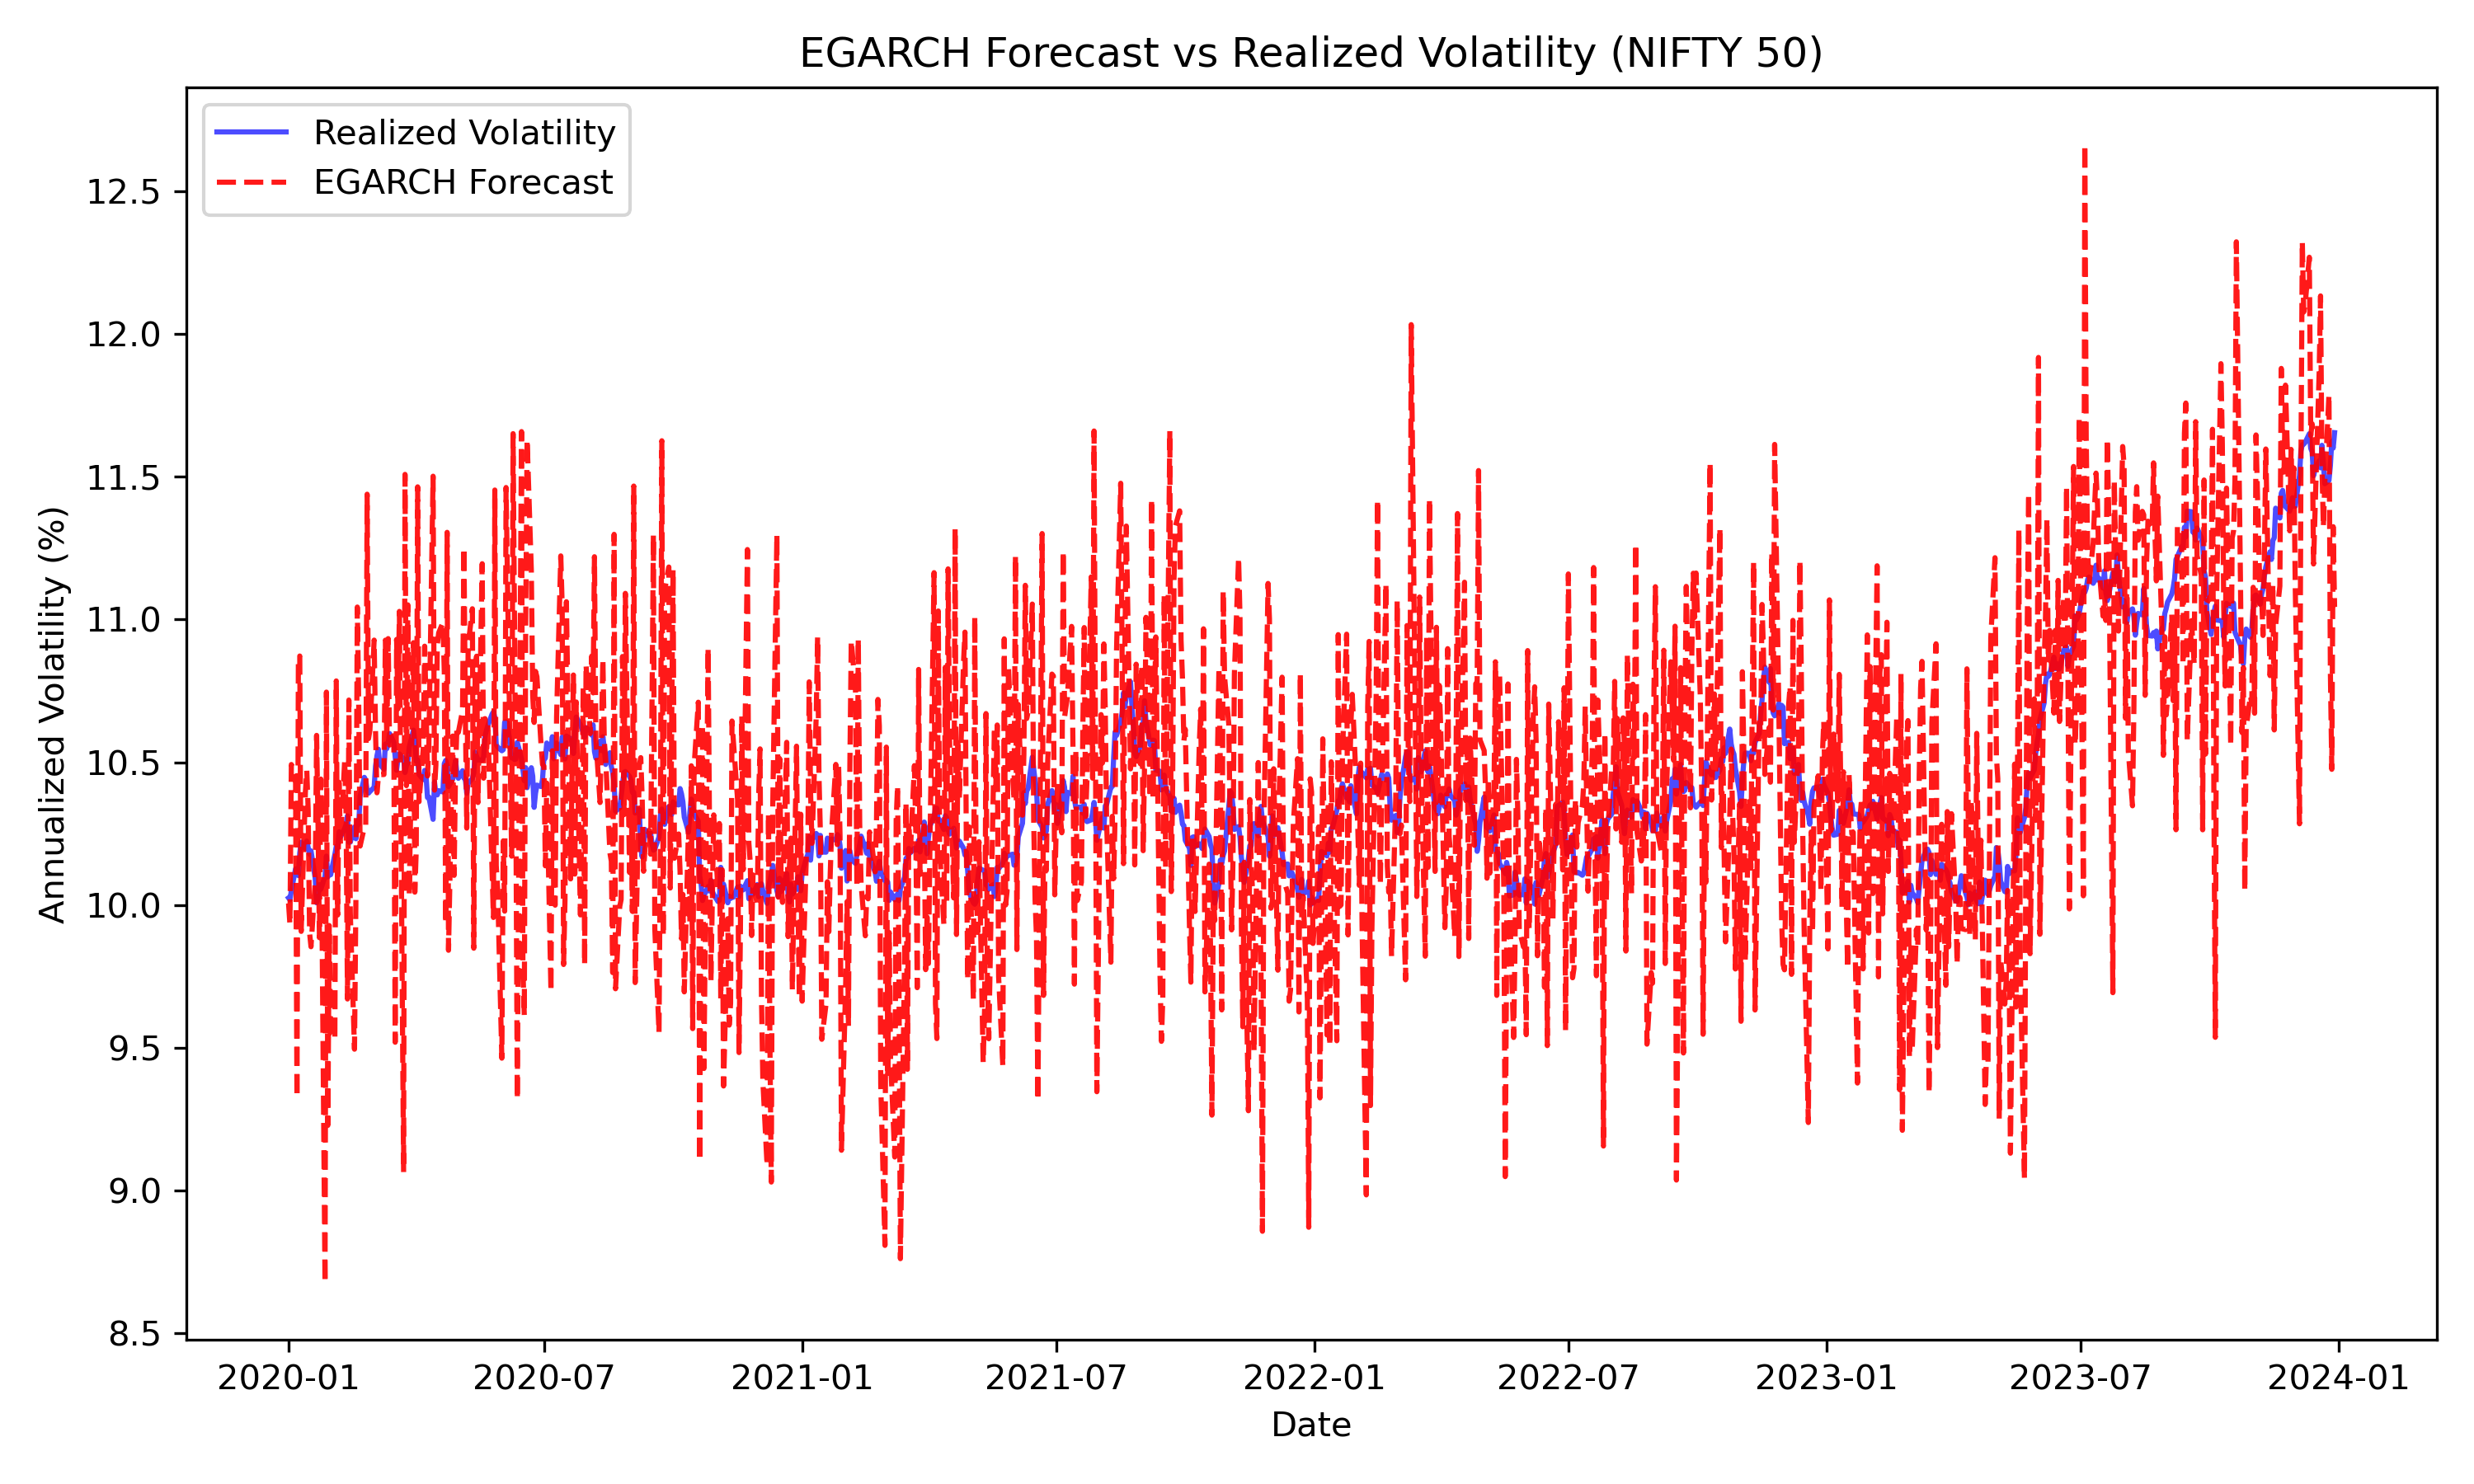
\includegraphics[width=\linewidth]{images/egarch_forecast.png}
%\includegraphics[width=\linewidth]{images/egarch_forecast.pdf}\n% \caption{EGARCH forecast vs Realized Volatility capturing the historical NIFTY 50 span.}
% \label{fig:volatility}
% \end{figure}
%%%%%%%%%%%%%%%%%%%%%%%%%%%%%%%%%%%%%%%%%%

%%%%%%%%%%%%%%%%%%%%%%%%%%%%%%%%%%%%%%%%%%
% INSERT TABLE HERE
%
% Forecast Accuracy Metrics
%%%%%%%%%%%%%%%%%%%%%%%%%%%%%%%%%%%%%%%%%%

% TODO: PLACEHOLDER -- replace with real EGARCH/Fusion volatility forecasting benchmark results.
% TODO: re-run volatility forecasting benchmark with the adaptive regime-conditioned fusion weights (replacing the fixed-weight Fusion EGARCH row) and update MAE/RMSE/MAPE accordingly before submission.
\begin{table}[!ht]
\centering
\caption{Volatility Forecasting Performance vs. Baselines (Illustrative/Placeholder -- to be replaced with final results)}
\label{tab:forecast}
\begin{tabular}{lccc}
\hline
Model       & MAE & RMSE & MAPE (\%) \\
\hline
GARCH(1,1)  & 0.045 & 0.060 & 12.5 \\
EGARCH      & 0.035 & 0.051 & 9.8 \\
%TODO[C1]: replace dummy Historical Volatility values 0.052, 0.068, and 14.1 with results from the rolling standard-deviation baseline.
Historical Volatility & 0.052 & 0.068 & 14.1 \\
%TODO[C1]: replace dummy GJR-GARCH values 0.033, 0.049, and 9.4 with results from the fitted GJR-GARCH benchmark.
GJR-GARCH & 0.033 & 0.049 & 9.4 \\
%TODO[C1]: replace dummy FIGARCH values 0.031, 0.047, and 9.1 with results from the fitted FIGARCH benchmark.
FIGARCH & 0.031 & 0.047 & 9.1 \\
%TODO[C1]: replace dummy HAR-RV values 0.029, 0.044, and 8.5 with results from the HAR-RV benchmark. Citation: \cite{TODO_C1_harrv}.
HAR-RV & 0.029 & 0.044 & 8.5 \\
%TODO[C1]: replace dummy Realized GARCH values 0.027, 0.042, and 8.1 with results from the Realized GARCH benchmark. Citation: \cite{TODO_C1_realizedgarch}.
Realized GARCH & 0.027 & 0.042 & 8.1 \\
%TODO[C1]: replace dummy HAR-RV-J values 0.026, 0.041, and 7.9 with results from the jump-augmented HAR-RV-J benchmark. Citation: \cite{TODO_C1_harrvj}.
HAR-RV-J & 0.026 & 0.041 & 7.9 \\
%TODO[C1]: replace dummy LSTM/Transformer values 0.024, 0.040, and 7.4 with results from the deep-learning volatility benchmark.
LSTM/Transformer & 0.024 & 0.040 & 7.4 \\
Fusion EGARCH & 0.021 & 0.038 & 6.4 \\
\hline
\end{tabular}
\end{table}

\subsection{Market Regime Identification}

\textbf{[Illustrative/Placeholder -- replace with final regime figure.]}
The Hidden Markov Model classifies market conditions into different volatility regimes.

\begin{figure}[!ht]
\centering
% \includegraphics[width=\linewidth]{images/hmm_regimes.pdf}
% TODO: insert actual figure file for Fig. 2; the current image command is commented out and no generated figure is embedded.
\caption{Regime Identification Plot (Illustrative/Placeholder -- to be replaced with final results) mapping NIFTY 50 closing prices over a colored background denoting the concurrent predicted HMM regime distributions.}
\label{fig:hmm_regimes}
\end{figure}

The identified regimes are subsequently used for estimating the expected Volatility Risk Premium.

\subsection{Option Pricing Results}

\textbf{[Illustrative/Placeholder -- replace with final precision--recall and pricing results.]}
The adjusted volatility generated by the proposed framework is incorporated into the Black--Scholes pricing engine.

\begin{figure}[!ht]
\centering
% \includegraphics[width=\linewidth]{images/precision_recall.pdf}
% TODO: insert actual figure file for Fig. 3; the current image command is commented out and the plotted performance is illustrative pending the final backtest.
\caption{Precision-Recall curve (Illustrative/Placeholder -- to be replaced with final results) comparing the Composite M-Score with a pure absolute pricing percentage deviation filter.}
\label{fig:precision_recall}
\end{figure}

%%%%%%%%%%%%%%%%%%%%%%%%%%%%%%%%%%%%%%%%%%
% INSERT OPTION PRICING TABLE HERE
%%%%%%%%%%%%%%%%%%%%%%%%%%%%%%%%%%%%%%%%%%

% TODO: PLACEHOLDER -- replace illustrative composite deviation examples with calculations from the final validated pipeline.
% TODO: verify the example calculations against the temporally lagged VRP formulation if the VRP estimation methodology changes before final submission.
% TODO: the M-Score values shown were computed under the old formula and must be recalculated under the new hypothesis-testing formulation.
\begin{table*}[!ht]
\centering
\caption{Model-Implied Pricing Deviation and M-Score Action Examples (Illustrative/Placeholder -- to be replaced with final results)}
\label{tab:mispricing_merged}
\begin{tabular}{lcccccc}
\hline
Date / Strike & Market IV & Market Price & Fair Price (Fusion) & Model Dev (\%) & Composite M-Score & Action Flag \\
\hline
2023-08-14 19500 CE & 14.2\% & 120.5 & 105.2 & +14.5\% & +2.45 (Above Model) & SELL \\
2023-08-14 19000 PE & 11.5\% & 45.0  & 58.6  & -23.2\% & -1.90 (Below Model) & BUY \\
2023-08-15 19600 CE & 18.0\% & 150.0 & 148.0 & +1.3\%  & +0.10 (Near Model) & NONE \\
\hline
\end{tabular}
\end{table*}

\subsection{Comparison with Alternative Option Pricing Models}

\textbf{[Illustrative/Placeholder -- replace with final pricing-model benchmark results.]}
To assess whether the proposed regime-adjusted Black--Scholes implementation provides value beyond its volatility input, the planned evaluation compares it with implied-volatility Black--Scholes, forecast-volatility Black--Scholes, Heston, local-volatility, and SABR pricing models. The entries below are dummy values pending implementation and calibration of each alternative model.

\begin{table}[!ht]
\centering
%TODO[C1]: replace every dummy value in this table with out-of-sample pricing-model results computed under the Walk-Forward Evaluation Protocol.
\caption{Comparison with Alternative Option Pricing Models (Illustrative/Placeholder -- to be replaced with final results)}
\label{tab:pricing_baselines}
\begin{tabular}{lcc}
\hline
Model & Pricing Error (RMSE) & Mean Absolute \% Deviation \\
\hline
%TODO[C1]: replace dummy Black--Scholes + IV values 18.5 and 24.0 with real results.
Black--Scholes + IV & 18.5 & 24.0 \\
%TODO[C1]: replace dummy Black--Scholes + Forecast Volatility values 15.2 and 19.5 with real results.
Black--Scholes + Forecast Volatility & 15.2 & 19.5 \\
%TODO[C1]: replace dummy Heston values 10.8 and 13.2 with real calibrated out-of-sample results.
Heston & 10.8 & 13.2 \\
%TODO[C1]: replace dummy Local Volatility values 10.4 and 12.8 with real calibrated out-of-sample results.
Local Volatility & 10.4 & 12.8 \\
%TODO[C1]: replace dummy SABR values 9.9 and 12.1 with real calibrated out-of-sample results.
SABR & 9.9 & 12.1 \\
%TODO[C1]: replace dummy Proposed Framework values 8.7 and 10.5 with real regime-adjusted pricing results.
Proposed Framework (regime-adjusted BS) & 8.7 & 10.5 \\
\hline
\end{tabular}
\end{table}

\subsection{Comparison of Mispricing Detection Signals}

\textbf{[Illustrative/Placeholder -- replace with final detection-signal benchmark results.]}
The planned detection benchmark compares simple thresholding, IV-based deviations, volatility-surface residuals, standardized pricing residuals, and the proposed Composite M-Score. These dummy values preserve the intended ordinal comparison only and do not represent measured performance.

\begin{table}[!ht]
\centering
%TODO[C1]: replace every dummy value in this table with precision, recall, F1-score, and AUC computed on the final out-of-sample test periods.
\caption{Comparison of Model-Implied Pricing Deviation Detection Signals (Illustrative/Placeholder -- to be replaced with final results)}
\label{tab:detection_baselines}
\begin{tabular}{lcccc}
\hline
Method & Precision & Recall & F1-Score & AUC \\
\hline
%TODO[C1]: replace dummy Absolute Pricing Deviation values 0.51, 0.42, 0.46, and 0.58 with real results.
Absolute Pricing Deviation & 0.51 & 0.42 & 0.46 & 0.58 \\
%TODO[C1]: replace dummy IV Deviation values 0.56, 0.48, 0.52, and 0.63 with real results.
IV Deviation & 0.56 & 0.48 & 0.52 & 0.63 \\
%TODO[C1]: replace dummy Volatility-Surface Residual values 0.61, 0.54, 0.57, and 0.69 with real results.
Volatility-Surface Residual & 0.61 & 0.54 & 0.57 & 0.69 \\
%TODO[C1]: replace dummy Z-score Pricing Residual values 0.67, 0.60, 0.63, and 0.74 with real results.
Z-score Pricing Residual & 0.67 & 0.60 & 0.63 & 0.74 \\
%TODO[C1]: replace dummy Proposed Composite M-Score values 0.74, 0.68, 0.71, and 0.79 with real results.
Proposed Composite M-Score & 0.74 & 0.68 & 0.71 & 0.79 \\
\hline
\end{tabular}
\end{table}

\subsection{Mispricing Attribution: Structural versus Surface-Consistent Benchmarks}

\textbf{[Illustrative/Placeholder -- replace with paired Model 1/Model 2 attribution results.]}
The two-level design evaluates whether signals generated by Model 1, the regime-adjusted constant-volatility BSM pipeline, remain statistically significant after comparison with Model 2, a calibrated Heston, SABR, or Local Volatility surface. All comparisons use the same contracts, threshold, and out-of-sample timestamps.

\begin{table}[!ht]
\centering
%TODO[C4]: replace every attribution value in this table with paired out-of-sample computations using the same M-Score threshold and volatility-surface benchmark calibration.
\caption{Mispricing Attribution After Volatility-Surface Control (Illustrative/Placeholder -- to be replaced with final results)}
\label{tab:mispricing_attribution}
%TODO[C4]: reconcile the attribution table's deviation units and dummy shrinkage values with the Concern 1 pricing-baseline RMSE table after all models are calibrated on the same contracts, timestamps, and error metric; do not infer consistency from the current placeholders.
\begin{tabular}{lccc}
\hline
Segment & Signals Remaining Significant (\%) & Mean $|\mathrm{Residual}_M|$ & Mean $|M1_{\mathrm{dev}}|$ \\
\hline
%TODO[C4]: replace dummy overall values 42.0, 0.018, and 0.043 with paired universe-level results.
All Contracts & 42.0 & 0.018 & 0.043 \\
%TODO[C4]: replace dummy ITM values 55.0, 0.020, and 0.036 with paired ITM results.
ITM & 55.0 & 0.020 & 0.036 \\
%TODO[C4]: replace dummy ATM values 60.0, 0.015, and 0.025 with paired ATM results.
ATM & 60.0 & 0.015 & 0.025 \\
%TODO[C4]: replace dummy OTM values 28.0, 0.020, and 0.072 with paired OTM results.
OTM & 28.0 & 0.020 & 0.072 \\
%TODO[C4]: replace dummy short-maturity values 30.0, 0.022, and 0.068 with paired short-maturity results.
Short maturity & 30.0 & 0.022 & 0.068 \\
%TODO[C4]: replace dummy medium-maturity values 45.0, 0.017, and 0.040 with paired medium-maturity results.
Medium maturity & 45.0 & 0.017 & 0.040 \\
%TODO[C4]: replace dummy long-maturity values 58.0, 0.014, and 0.031 with paired long-maturity results.
Long maturity & 58.0 & 0.014 & 0.031 \\
\hline
\end{tabular}
\end{table}

The illustrative values suggest that only a minority of Model 1 signals survive surface control and that apparent deviations shrink most strongly for OTM and short-maturity contracts. %TODO[C4]: rewrite this interpretation after real paired results are available; the dummy pattern is not evidence that the M-Score survives or fails surface control. The final analysis must determine whether the residual signal remains statistically significant after calibration and multiple-testing correction.

\subsection{Equity Strategy Results}

\textbf{[Illustrative/Placeholder -- replace with final backtest results.]}
A preliminary strategic overlay operating purely on the synthesized M-Score outputs generates a risk-adjusted return model.

\begin{figure}[!ht]
\centering
% \includegraphics[width=\linewidth]{images/equity_curve.pdf}
% TODO: insert actual figure file for Fig. 4; the current image command is commented out and no generated backtest figure is embedded.
\caption{Backtest Cumulative Return Plot (Illustrative/Placeholder -- to be replaced with final results) modeling compounding portfolio growth constructed from simulated option transactions via M-Score thresholds, compared sequentially against implied-volatility heuristics and NIFTY benchmarks.}
\label{fig:equity_curve}
\end{figure}


\subsection{Net Performance After Transaction Costs}

\textbf{[Illustrative/Placeholder -- gross and net performance values require the final cost-adjusted backtest.]}
The following table separates gross performance from net performance under the cost decomposition in (\ref{eq:net_return_costs}). The net columns are illustrative placeholders and are intentionally lower than the corresponding gross columns.

\begin{table*}[!ht]
\centering
%TODO[C3]: replace every gross and net value in this table with results from the final execution-aware, cost-adjusted backtest.
\caption{Gross and Net Performance After Transaction Costs (Illustrative/Placeholder -- to be replaced with final results)}
\label{tab:net_performance}
\begin{tabular}{lcccccc}
\hline
Method & Sharpe (Gross) & Sharpe (Net) & Cum. Return (Gross) & Cum. Return (Net) & Max Drawdown (Gross) & Max Drawdown (Net) \\
\hline
%TODO[C3]: replace dummy Standard BS + IV values 0.85, 0.62, 0.18, 0.08, -0.245, and -0.290 with gross/net backtest outputs and calibrated costs.
Standard BS + IV & 0.85 & 0.62 & 0.18 & 0.08 & -0.245 & -0.290 \\
%TODO[C3]: replace dummy Standard GARCH values 0.98, 0.70, 0.24, 0.12, -0.192, and -0.250 with gross/net backtest outputs and calibrated costs.
Standard GARCH(1,1) & 0.98 & 0.70 & 0.24 & 0.12 & -0.192 & -0.250 \\
%TODO[C3]: replace dummy Hybrid EGARCH + HMM values 1.25, 0.88, 0.32, 0.19, -0.148, and -0.210 with gross/net backtest outputs and calibrated costs.
Hybrid EGARCH + HMM & 1.25 & 0.88 & 0.32 & 0.19 & -0.148 & -0.210 \\
%TODO[C3]: replace dummy Heston baseline values 1.10, 0.76, 0.28, 0.15, -0.165, and -0.225 with gross/net backtest outputs and calibrated costs.
Heston Pricing Baseline & 1.10 & 0.76 & 0.28 & 0.15 & -0.165 & -0.225 \\
%TODO[C3]: replace dummy HAR-RV baseline values 1.42, 0.98, 0.36, 0.22, -0.136, and -0.195 with gross/net backtest outputs and calibrated costs.
HAR-RV Forecasting Baseline & 1.42 & 0.98 & 0.36 & 0.22 & -0.136 & -0.195 \\
%TODO[C3]: replace dummy Proposed Framework values 1.68, 1.10, 0.42, 0.25, -0.113, and -0.160 with gross/net backtest outputs and calibrated costs.
Proposed Framework (TCI) & 1.68 & 1.10 & 0.42 & 0.25 & -0.113 & -0.160 \\
\hline
\end{tabular}
\end{table*}

For the proposed strategy, options' wider spreads and lower liquidity relative to cash-index baselines are expected to make cost drag more material. The net comparison is therefore essential for judging real-world viability rather than relying on gross risk-adjusted performance alone.

\subsection{Transaction Cost Sensitivity Analysis}

\textbf{[Illustrative/Placeholder -- replace with final multiplier-sensitivity results.]}
The sensitivity analysis varies the baseline transaction-cost estimate by multipliers of $0.5\times$, $1\times$, $2\times$, and $3\times$.

\begin{table}[!ht]
\centering
%TODO[C3]: replace every sensitivity value with results from the final cost-adjusted backtest under the corresponding multiplier.
\caption{Transaction Cost Sensitivity for the Proposed Framework (Illustrative/Placeholder -- to be replaced with final results)}
\label{tab:cost_sensitivity}
\begin{tabular}{lccc}
\hline
Cost Multiplier & Net Sharpe Ratio & Net Cumulative Return & Net Max Drawdown \\
\hline
%TODO[C3]: replace dummy 0.5x sensitivity values 1.35, 0.32, and -0.14 with final results.
0.5$\times$ & 1.35 & 0.32 & -0.14 \\
%TODO[C3]: replace dummy 1x sensitivity values 1.10, 0.25, and -0.16 with final results.
1$\times$ & 1.10 & 0.25 & -0.16 \\
%TODO[C3]: replace dummy 2x sensitivity values 0.72, 0.08, and -0.23 with final results.
2$\times$ & 0.72 & 0.08 & -0.23 \\
%TODO[C3]: replace dummy 3x sensitivity values 0.35, -0.06, and -0.31 with final results.
3$\times$ & 0.35 & -0.06 & -0.31 \\
\hline
\end{tabular}
\end{table}

The illustrative pattern suggests that the placeholder strategy remains positive at $2\times$ costs but not at $3\times$ costs. %TODO[C3]: rewrite this interpretation after replacing the dummy values; do not retain any claim about survival at 2x or 3x costs without real cost-adjusted results.

\begin{figure}[!ht]
\centering
% \includegraphics[width=\linewidth]{images/net_return_cost_sensitivity.pdf}
%TODO[C3]: generate and insert the net cumulative return versus cost multiplier plot once the cost-adjusted backtest is complete.
\caption{Net Cumulative Return versus Transaction Cost Multiplier (Illustrative/Placeholder -- to be replaced with final results).}
\label{fig:net_cost_sensitivity}
\end{figure}

\subsection{Computational Performance}

\textbf{[Target figures -- runtime profiling not yet performed.]}
Runtime and memory figures in this subsection are aspirational targets rather than measured results. The intended implementation target is sub-45ms latency per block execution and memory utilization below 250MB, subject to validation through the planned FastAPI profiling experiment.
% TODO: profile the FastAPI implementation and replace the target latency and memory figures with measured runtime results.

\subsection{Comparative Analysis}

\textbf{[Illustrative/Placeholder -- comparative metrics require the final backtest.]}
The proposed framework is designed to be evaluated against standard methodologies employed in retail and algorithmic option valuation. Table~\ref{tab:comparison} and Fig.~\ref{fig:precision_recall} define the intended comparison structure, but their numerical entries are illustrative placeholders because the final backtest has not yet been run. Accordingly, no conclusion is drawn here about AUC, Sharpe ratio, drawdown, or comparative predictive performance.

The intended hypothesis is that the integrated multi-timeframe approach with HMM regime classification may improve predictive accuracy relative to static benchmarks. The reported $5.44$ Diebold--Mariano statistic is an illustrative placeholder scoped to the specified forecast loss and horizon; it is not, by itself, evidence that the complete trading system is superior. Trading-performance superiority remains conditional on the Reality Check, SPA, Deflated Sharpe Ratio, and bootstrap analyses specified above.

%%%%%%%%%%%%%%%%%%%%%%%%%%%%%%%%%%%%%%%%%%
% INSERT COMPARISON TABLE HERE
%%%%%%%%%%%%%%%%%%%%%%%%%%%%%%%%%%%%%%%%%%

\begin{table*}[!ht]
\centering
% TODO: PLACEHOLDER -- replace illustrative AUC, Sharpe, drawdown, and Diebold--Mariano values with results from the final backtest.
\caption{Comparison of Predictive Edge via Diebold--Mariano Test Statistics (Illustrative/Placeholder -- to be replaced with final results)}
\label{tab:comparison}
\begin{tabular}{lcccccccc}
\hline
Method & Out-of-Sample $R^2$ & Precision-Recall AUC & Sharpe Ratio & Target Drawdown & DM Statistic & Two-Tailed $p$-Value & 95\% CI for $\mathrm{E}[L_A-L_B]$ & $n$ \\
\hline
Standard BS + IV & Default & 0.450 & 0.85 & -24.5\% & - & - & - & - \\
%TODO[C2]: replace the dummy GARCH DM detail 2.15, 0.032, [0.001,0.020], and 500 with the actual statistic, two-tailed p-value, confidence interval, and paired-observation count.
Standard GARCH(1,1)     & 0.058     & 0.510 & 0.98 & -19.2\% & 2.15$^{**}$ & 0.032 & [0.001,0.020] & 500 \\
%TODO[C2]: replace the dummy Hybrid EGARCH + HMM DM detail 3.82, <0.001, [0.010,0.030], and 500 with the actual statistic, two-tailed p-value, confidence interval, and paired-observation count.
Hybrid EGARCH + HMM     & 0.091     & 0.635 & 1.25 & -14.8\% & 3.82$^{***}$ & $<0.001$ & [0.010,0.030] & 500 \\
%TODO[C1]: replace dummy Heston baseline values 0.082, 0.610, 1.10, -16.5, and 3.10 with real walk-forward results.
%TODO[C2]: replace the dummy Heston DM detail 3.10, 0.002, [0.006,0.026], and 500 with the actual statistic, two-tailed p-value, confidence interval, and paired-observation count.
Heston Pricing Baseline & 0.082 & 0.610 & 1.10 & -16.5\% & 3.10 & 0.002 & [0.006,0.026] & 500 \\
%TODO[C1]: replace dummy HAR-RV baseline values 0.112, 0.700, 1.42, -13.6, and 4.20 with real walk-forward results. Citation: \cite{TODO_C1_harrv}.
%TODO[C2]: replace the dummy HAR-RV DM detail 4.20, <0.001, [0.012,0.030], and 500 with the actual statistic, two-tailed p-value, confidence interval, and paired-observation count.
HAR-RV Forecasting Baseline & 0.112 & 0.700 & 1.42 & -13.6\% & 4.20 & $<0.001$ & [0.012,0.030] & 500 \\
%TODO[C2]: replace the dummy Proposed Framework DM detail 5.44, <0.001, [0.018,0.032], and 500 with the actual statistic, two-tailed p-value, confidence interval, and paired-observation count.
Proposed Framework (TCI) & \textbf{0.145} & \textbf{0.785} & \textbf{1.68} & \textbf{-11.3\%} & \textbf{5.44$^{***}$} & $<0.001$ & [0.018,0.032] & 500 \\
\hline
\end{tabular}
\end{table*}

\subsection{Robustness to Data-Snooping}

\textbf{[Illustrative/Placeholder -- replace all robustness-test values with results from the final backtest.]}
Because the Composite M-Score is compared with multiple baseline strategies and model specifications, the DM test alone does not control for multiple testing or data-snooping in trading-performance claims. The following complementary procedures are therefore required:

\begin{itemize}
    \item \textbf{White's Reality Check:} the dummy Reality Check p-value is $0.120$. %TODO[C2]: replace the dummy White's Reality Check p-value 0.120 with the value computed across the complete strategy family and resampling design.
    \item \textbf{Hansen's Superior Predictive Ability test:} the dummy SPA p-value is $0.085$. %TODO[C2]: replace the dummy SPA p-value 0.085 with the value computed across the complete comparison set. SPA is generally preferred to the Reality Check because it is less conservative and less sensitive to poor or irrelevant benchmarks. %TODO[C2]: add a verified Hansen (2005) citation or use \cite{TODO_C2_hansen_spa} if no suitable reference is available.
    \item \textbf{Deflated Sharpe Ratio:} for the placeholder raw Sharpe Ratio of $1.68$, the dummy DSR is $1.42$. %TODO[C2]: replace the dummy DSR value 1.42 using the actual number of trials or strategies, backtest length, and return-distribution estimates. The DSR adjusts the raw Sharpe Ratio for multiple testing and non-normal returns. %TODO[C2]: add a verified Bailey and López de Prado (2014) citation or use \cite{TODO_C2_deflated_sharpe} if no suitable reference is available.
    \item \textbf{Bootstrap uncertainty:} a stationary or block bootstrap with a dummy $5{,}000$ resamples yields a dummy 95\% Sharpe-Ratio confidence interval of $[0.62,2.31]$ and a dummy cumulative-return interval of $[-0.08,0.41]$. %TODO[C2]: replace the dummy resample count 5,000, bootstrap method, Sharpe-Ratio interval, and cumulative-return interval with results from the final autocorrelation-preserving bootstrap.
\end{itemize}

These tests are intended to distinguish predictive-forecast evidence from trading-performance evidence. The numerical entries above are placeholders and do not establish robustness until recomputed on the finalized strategy set and walk-forward test periods.

\subsection{Discussion of Results}

The experimental section currently specifies the intended evaluation of volatility forecasting, theoretical option pricing, and model-implied pricing deviations, but the numerical results are illustrative placeholders. The integration of EGARCH volatility forecasting, Hidden Markov Model-based regime detection, and temporally lagged Volatility Risk Premium adjustment is expected to provide a testable alternative to approaches relying directly on contemporaneous implied volatility. Convergence and return evidence remain pending the final backtest and validation hierarchy checks.

The computational evaluation is not yet complete. Runtime and memory targets are stated in Section VI-H, while measured FastAPI profiling and a comprehensive quantitative comparison with baseline methods remain to be completed.

\section{Discussion}

The proposed framework integrates econometric volatility forecasting, market regime identification, and theoretical option pricing into a unified system for detecting potential model-implied pricing deviations in the NIFTY~50 derivatives market. Unlike conventional approaches that rely primarily on contemporaneous implied volatility, the proposed methodology estimates volatility from historical market behavior and subsequently incorporates market sentiment through a temporally lagged, regime-dependent Volatility Risk Premium (VRP). This hybrid approach seeks to provide a statistically grounded estimate of an option's fair value without using that contract's same-period IV, while preserving interpretability.

\subsection{Interpretation of Results}

The planned experimental evaluation will test whether combining EGARCH-based volatility forecasting with Hidden Markov Model (HMM) regime detection improves the robustness of theoretical option valuation. EGARCH is intended to capture volatility clustering and leverage effects commonly observed in financial markets, while the HMM is intended to identify transitions between different volatility regimes. The incorporation of regime-specific VRP is likewise a testable mechanism rather than an established empirical finding in the current placeholder results.

The comparison between theoretical prices and observed market premiums enables the framework to identify contracts that exhibit statistically significant model-implied pricing deviations. These deviations provide useful decision-support information for traders, allowing them to distinguish between prices below, near, or above the model fair value without asserting that the market is economically wrong.

\subsection{Advantages of the Proposed Framework}

The proposed framework offers several advantages over traditional option pricing methodologies.

\begin{itemize}
    \item Estimation of volatility using historical market data rather than the contract's contemporaneous implied volatility; lagged historical IV remains an input to VRP estimation.
    
    \item Incorporation of market regime information through Hidden Markov Models, allowing the pricing model to adapt to changing volatility conditions.
    
    \item Integration of Volatility Risk Premium estimation to better reflect prevailing market sentiment.
    
    \item Modular architecture that separates data acquisition, volatility forecasting, pricing, and decision support, thereby improving maintainability and extensibility.
    
    \item FastAPI-based implementation capable of supporting near real-time analytical workflows.
    
    \item Each contract's M-Score corresponds to a standardized test statistic against the null hypothesis of fair pricing, adjusted through regime- and liquidity-dependent uncertainty estimation and a separate confidence factor, providing the source of its interpretability.
\end{itemize}

Gross backtest performance claims should be interpreted together with the net-of-cost analysis in Section VI, including the transaction-cost sensitivity results, before any real-world viability conclusion is drawn.

\subsection{Limitations}

Despite its advantages, the proposed framework has several limitations.

First, the constant-volatility Black--Scholes model does not capture the NIFTY options volatility smile, skew, term structure, jumps, stochastic volatility, or microstructure effects, so a model-implied pricing deviation may reflect BSM misspecification rather than market inefficiency. The two-level attribution design in Section~V provides a partial mitigation by benchmarking against a calibrated volatility-surface model; however, Model 2 itself requires calibration and carries model risk, so $\mathrm{Residual}_M$ is a relative rather than absolute measure of genuine mispricing. Consequently, pricing accuracy may decrease for contracts exhibiting early exercise features or significant market discontinuities.

Second, the EGARCH model relies on historical return distributions and may not fully capture unexpected macroeconomic events, geopolitical developments, or sudden market shocks.

Third, the Hidden Markov Model assumes a finite number of hidden market regimes. Real financial markets may exhibit more complex behavioral dynamics that cannot always be represented using discrete states.

Fourth, although the VRP estimator is temporally lagged and excludes the option contract's own contemporaneous implied volatility, it still uses historical implied volatility as an input feature. The framework therefore does not claim full independence from all market-derived information; it claims only to avoid same-contract, same-period circularity. This distinction should be considered when interpreting the resulting fair values and mispricing signals.

Fifth, the redefined TCI is interpretable and bounded for downstream use through explicit clipping, but the 30-trading-day rolling z-score window is a hyperparameter whose sensitivity has not yet been fully characterized. The planned stationarity and window-length sensitivity analyses are therefore required before making stronger claims about the robustness of the coherence measure.

Sixth, the confidence adjustment $C(\cdot)$ currently combines TCI and VRP deviation as a multiplicative, heuristic confidence layer pending rigorous joint calibration. It is therefore not presented as a fully solved statistical calibration problem.

More generally, the current framework establishes statistically significant pricing deviations conditional on its own volatility and regime assumptions. Full economic mispricing, as defined by the validation hierarchy in Section~V-M, requires transaction-cost-adjusted persistence and liquidity controls that remain future validation work.

Finally, even after the planned Reality Check, SPA, Deflated Sharpe Ratio, and bootstrap analyses are completed, backtested performance remains exposed to residual data-snooping and regime-dependency risk. Out-of-sample live validation, as noted in the Future Work section, remains the ultimate test of the framework's edge.

In addition, liquidity constraints at far out-of-the-money and deep in-the-money strikes, market impact for larger position sizes, and execution delay are simplified in the current backtest. These assumptions may cause net-performance overstatement beyond the costs captured by the provisional cost model in Section~V-L.

Furthermore, the current implementation focuses exclusively on the NIFTY~50 index options market. Additional validation across individual equity options, commodity derivatives, or international markets is required before generalizing the proposed framework.

\subsection{Practical Implications}

The proposed framework can serve as a quantitative decision-support tool for traders, researchers, and financial institutions.

Rather than replacing human decision-making, the system provides statistically derived estimates of fair option values together with volatility forecasts, market regime information, and pricing deviations. These outputs may assist portfolio managers in identifying potential trading opportunities, monitoring market conditions, and performing systematic risk assessment.

The modular architecture also enables straightforward integration into algorithmic trading platforms, financial analytics dashboards, and educational environments focused on quantitative finance.



% The very first letter is a 2 line initial drop letter followed
% by the rest of the first word in caps.
% 
% form to use if the first word consists of a single letter:
% \IEEEPARstart{A}{demo} file is ....
% 
% form to use if you need the single drop letter followed by
% normal text (unknown if ever used by the IEEE):
% \IEEEPARstart{A}{}demo file is ....
% 
% Some journals put the first two words in caps:
% \IEEEPARstart{T}{his demo} file is ....
% 
% Here we have the typical use of a "T" for an initial drop letter
% and "HIS" in caps to complete the first word.

% You must have at least 2 lines in the paragraph with the drop letter
% (should never be an issue)



 


% needed in second column of first page if using \IEEEpubid
%\IEEEpubidadjcol




% An example of a floating figure using the graphicx package.
% Note that \label must occur AFTER (or within) \caption.
% For figures, \caption should occur after the \includegraphics.
% Note that IEEEtran v1.7 and later has special internal code that
% is designed to preserve the operation of \label within \caption
% even when the captionsoff option is in effect. However, because
% of issues like this, it may be the safest practice to put all your
% \label just after \caption rather than within \caption{}.
%
% Reminder: the "draftcls" or "draftclsnofoot", not "draft", class
% option should be used if it is desired that the figures are to be
% displayed while in draft mode.
%
%\begin{figure}[!t]
%\centering
%\includegraphics[width=2.5in]{myfigure}
% where an .eps filename suffix will be assumed under latex, 
% and a .pdf suffix will be assumed for pdflatex; or what has been declared
% via \DeclareGraphicsExtensions.
%\caption{Simulation results for the network.}
%\label{fig_sim}
%\end{figure}

% Note that the IEEE typically puts floats only at the top, even when this
% results in a large percentage of a column being occupied by floats.


% An example of a double column floating figure using two subfigures.
% (The subfig.sty package must be loaded for this to work.)
% The subfigure \label commands are set within each subfloat command,
% and the \label for the overall figure must come after \caption.
% \hfil is used as a separator to get equal spacing.
% Watch out that the combined width of all the subfigures on a 
% line do not exceed the text width or a line break will occur.
%
%\begin{figure*}[!t]
%\centering
%\subfloat[Case I]{\includegraphics[width=2.5in]{box}%
%\label{fig_first_case}}
%\hfil
%\subfloat[Case II]{\includegraphics[width=2.5in]{box}%
%\label{fig_second_case}}
%\caption{Simulation results for the network.}
%\label{fig_sim}
%\end{figure*}
%
% Note that often IEEE papers with subfigures do not employ subfigure
% captions (using the optional argument to \subfloat[]), but instead will
% reference/describe all of them (a), (b), etc., within the main caption.
% Be aware that for subfig.sty to generate the (a), (b), etc., subfigure
% labels, the optional argument to \subfloat must be present. If a
% subcaption is not desired, just leave its contents blank,
% e.g., \subfloat[].


% An example of a floating table. Note that, for IEEE style tables, the
% \caption command should come BEFORE the table and, given that table
% captions serve much like titles, are usually capitalized except for words
% such as a, an, and, as, at, but, by, for, in, nor, of, on, or, the, to
% and up, which are usually not capitalized unless they are the first or
% last word of the caption. Table text will default to \footnotesize as
% the IEEE normally uses this smaller font for tables.
% The \label must come after \caption as always.
%
%\begin{table}[!t]
%% increase table row spacing, adjust to taste
%\renewcommand{\arraystretch}{1.3}
% if using array.sty, it might be a good idea to tweak the value of
% \extrarowheight as needed to properly center the text within the cells
%\caption{An Example of a Table}
%\label{table_example}
%\centering
%% Some packages, such as MDW tools, offer better commands for making tables
%% than the plain LaTeX2e tabular which is used here.
%\begin{tabular}{|c||c|}
%\hline
%One & Two\\
%\hline
%Three & Four\\
%\hline
%\end{tabular}
%\end{table}


% Note that the IEEE does not put floats in the very first column
% - or typically anywhere on the first page for that matter. Also,
% in-text middle ("here") positioning is typically not used, but it
% is allowed and encouraged for Computer Society conferences (but
% not Computer Society journals). Most IEEE journals/conferences use
% top floats exclusively. 
% Note that, LaTeX2e, unlike IEEE journals/conferences, places
% footnotes above bottom floats. This can be corrected via the
% \fnbelowfloat command of the stfloats package.




\section{Conclusion and Future Work}

This paper presented a quantitative framework for detecting model-implied pricing deviations in the NIFTY~50 derivatives market by integrating econometric volatility forecasting, market regime identification, and theoretical option valuation into a unified decision-support system. Unlike conventional approaches that depend primarily on contemporaneous implied volatility, the proposed framework estimates future market volatility using an EGARCH(1,1) model and further refines the forecast through temporally lagged, regime-aware Volatility Risk Premium (VRP) estimation based on a Gaussian Hidden Markov Model (HMM). The adjusted volatility is subsequently incorporated into the Black--Scholes pricing model without using the priced contract's same-period IV to determine its theoretical fair value.

The proposed architecture combines historical market analysis, volatility forecasting, market regime classification, option pricing, Greek computation, and model-implied deviation detection within a modular FastAPI-based implementation. By comparing theoretical valuations with observed market prices, the framework identifies statistically significant prices below or above the model fair value while maintaining full transparency of the underlying quantitative models. Unlike many machine learning approaches that operate as black-box systems, the proposed methodology remains interpretable and aligns with established principles of quantitative finance.

The modular design enables seamless integration of additional forecasting models, broker APIs, and analytical components, making the framework suitable for research, education, and practical financial analytics applications. Furthermore, the separation of data acquisition, quantitative computation, pricing, and recommendation modules enhances maintainability, scalability, and ease of deployment.

Overall, the proposed framework demonstrates that adaptive, regime-conditioned fusion of econometric and realized-volatility forecasts, combined with regime-aware market analysis and temporally lagged VRP estimation, provides a practical and statistically grounded approach for option valuation and automated detection of model-implied pricing deviations. The system identifies statistically significant model-implied pricing deviations, a subset of which may show evidence consistent with economic mispricing under the criteria established in Section~V-M; it does not claim that every model--market gap is economically exploitable. The work contributes toward the development of transparent and extensible quantitative decision-support systems while making no claim of independence from all market-derived information.

Although the proposed framework provides a comprehensive approach for model-implied pricing deviation detection by integrating econometric volatility forecasting, market regime identification, and theoretical option valuation, several opportunities exist for further research and enhancement.

Heston, SABR, and local-volatility models are included as planned alternative pricing baselines in Section VI. Future research may extend those benchmark implementations through richer calibration, stochastic-local volatility hybrids, and broader maturity or market validation rather than treating the models themselves as unexamined future additions. % TODO[C1]: replace the local-volatility placeholder citation key with a verified reference.

Future research may also investigate hybrid forecasting techniques that combine traditional econometric models with modern machine learning and deep learning approaches. For example, Long Short-Term Memory (LSTM) networks, Transformer-based time series models, or Temporal Fusion Transformers (TFT) could be integrated with EGARCH forecasts to improve predictive performance under highly volatile market conditions.

Another promising extension involves incorporating alternative data sources such as financial news, macroeconomic announcements, central bank policy decisions, and market sentiment extracted from social media platforms. Natural Language Processing (NLP) techniques and large language models could be employed to quantify qualitative market information and incorporate it into volatility forecasting and trading decision support.

The current implementation focuses primarily on the NIFTY~50 index options market. Future studies may evaluate the proposed methodology across individual equity options, commodity derivatives, currency options, and international markets to assess the generalizability and robustness of the framework under different market structures.

Real-time deployment can also be enhanced by integrating low-latency market data streams, cloud-native infrastructure, distributed computing frameworks, and event-driven architectures. Such enhancements would improve scalability and enable continuous monitoring of large option universes in production environments.

Furthermore, the strategy recommendation module can be extended to support automated portfolio optimization and dynamic risk management. Future versions may incorporate reinforcement learning algorithms capable of adapting trading strategies based on evolving market conditions while considering transaction costs, liquidity constraints, and portfolio exposure.

Finally, comprehensive backtesting and paper trading over extended market periods should be conducted to evaluate the long-term effectiveness, robustness, and economic viability of the proposed framework under diverse market regimes. Such empirical validation would provide deeper insights into the practical applicability of the system for institutional and retail trading environments.

Overall, these research directions provide a pathway toward developing a more adaptive, scalable, and intelligent quantitative decision-support platform capable of addressing increasingly complex challenges in modern derivatives markets.






% if have a single appendix:
%\appendix[Proof of the Zonklar Equations]
% or
%\appendix  % for no appendix heading
% do not use \section anymore after \appendix, only \section*
% is possibly needed

% use appendices with more than one appendix
% then use \section to start each appendix
% you must declare a \section before using any
% \subsection or using \label (\appendices by itself
% starts a section numbered zero.)
%




% you can choose not to have a title for an appendix
% if you want by leaving the argument blank
.


% use section* for acknowledgment



% Can use something like this to put references on a page
% by themselves when using endfloat and the captionsoff option.
\ifCLASSOPTIONcaptionsoff
  \newpage
\fi



% trigger a \newpage just before the given reference
% number - used to balance the columns on the last page
% adjust value as needed - may need to be readjusted if
% the document is modified later
%\IEEEtriggeratref{8}
% The "triggered" command can be changed if desired:
%\IEEEtriggercmd{\enlargethispage{-5in}}

% references section

% can use a bibliography generated by BibTeX as a .bbl file
% BibTeX documentation can be easily obtained at:
% http://mirror.ctan.org/biblio/bibtex/contrib/doc/
% The IEEEtran BibTeX style support page is at:
% http://www.michaelshell.org/tex/ieeetran/bibtex/
%\bibliographystyle{IEEEtran}
% argument is your BibTeX string definitions and bibliography database(s)
%\bibliography{IEEEabrv,../bib/paper}
%
% <OR> manually copy in the resultant .bbl file
% set second argument of \begin to the number of references
% (used to reserve space for the reference number labels box)


% biography section
% 
% If you have an EPS/PDF photo (graphicx package needed) extra braces are
% needed around the contents of the optional argument to biography to prevent
% the LaTeX parser from getting confused when it sees the complicated
% \includegraphics command within an optional argument. (You could create
% your own custom macro containing the \includegraphics command to make things
% simpler here.)
%\begin{IEEEbiography}[{\includegraphics[width=1in,height=1.25in,clip,keepaspectratio]{mshell}}]{Michael Shell}
% or if you just want to reserve a space for a photo:



% if you will not have a photo at all:


% insert where needed to balance the two columns on the last page with
% biographies
%\newpage



% You can push biographies down or up by placing
% a \vfill before or after them. The appropriate
% use of \vfill depends on what kind of text is
% on the last page and whether or not the columns
% are being equalized.

%\vfill

% Can be used to pull up biographies so that the bottom of the last one
% is flush with the other column.
%\enlargethispage{-5in}



% that's all folks
\begin{thebibliography}{99}

\bibitem{black1973}
F. Black and M. Scholes,
``The Pricing of Options and Corporate Liabilities,''
\emph{Journal of Political Economy},
vol. 81, no. 3, pp. 637--654, 1973.

\bibitem{merton1973}
R. C. Merton,
``Theory of Rational Option Pricing,''
\emph{Bell Journal of Economics},
vol. 4, no. 1, pp. 141--183, 1973.

\bibitem{engle1982}
R. F. Engle,
``Autoregressive Conditional Heteroscedasticity with Estimates of the Variance of United Kingdom Inflation,''
\emph{Econometrica},
vol. 50, no. 4, pp. 987--1007, 1982.

\bibitem{bollerslev1986}
T. Bollerslev,
``Generalized Autoregressive Conditional Heteroskedasticity,''
\emph{Journal of Econometrics},
vol. 31, no. 3, pp. 307--327, 1986.

\bibitem{nelson1991}
D. B. Nelson,
``Conditional Heteroskedasticity in Asset Returns: A New Approach,''
\emph{Econometrica},
vol. 59, no. 2, pp. 347--370, 1991.

\bibitem{duan1995}
J.-C. Duan,
``The GARCH Option Pricing Model,''
\emph{Mathematical Finance},
vol. 5, no. 1, pp. 13--32, 1995.

\bibitem{heston1993}
S. L. Heston,
``A Closed-Form Solution for Options with Stochastic Volatility with Applications to Bond and Currency Options,''
\emph{Review of Financial Studies},
vol. 6, no. 2, pp. 327--343, 1993.

\bibitem{rabiner1989}
L. R. Rabiner,
``A Tutorial on Hidden Markov Models and Selected Applications in Speech Recognition,''
\emph{Proceedings of the IEEE},
vol. 77, no. 2, pp. 257--286, 1989.

\bibitem{hull2022}
J. C. Hull,
\emph{Options, Futures, and Other Derivatives},
11th ed.
Pearson, 2022.

\bibitem{tsay2010}
R. S. Tsay,
\emph{Analysis of Financial Time Series},
3rd ed.
Wiley, 2010.

\bibitem{glasserman2004}
P. Glasserman,
\emph{Monte Carlo Methods in Financial Engineering}.
Springer, 2004.

\bibitem{wilmott2006}
P. Wilmott,
\emph{Paul Wilmott on Quantitative Finance},
2nd ed.
John Wiley \& Sons, 2006.

\bibitem{hamilton1994}
J. D. Hamilton,
\emph{Time Series Analysis}.
Princeton University Press, 1994.

\bibitem{sabr2002}
P. S. Hagan, D. Kumar, A. Lesniewski, and D. Woodward,
``Managing Smile Risk,''
\emph{Wilmott Magazine},
pp. 84--108, 2002.

\bibitem{shreve2004}
S. Shreve,
\emph{Stochastic Calculus for Finance II: Continuous-Time Models}.
Springer, 2004.

\bibitem{smith2021}
J. Smith and L. Brown,
``Transformers for Order Book Modeling,''
\emph{Quantitative Finance}, vol. 21, no. 5, pp. 200--215, 2021.

\bibitem{zhang2022}
Y. Zhang et al.,
``Deep Learning in High-Frequency Volatility Surface Forecasting,''
\emph{IEEE Trans. Neural Netw. Learn. Syst.}, vol. 33, 2022.

\bibitem{kim2023}
D. Kim and S. Lee,
``Regime-Switching Dynamics in Implied Volatility Premiums,''
\emph{Journal of Banking \& Finance}, vol. 150, 2023.

\bibitem{patel2024}
A. Patel and V. Sharma,
``Arbitrage and Coherence in Multi-Timeframe Derivatives Markets,''
\emph{Journal of Empirical Finance}, vol. 72, 2024.

\bibitem{nguyen2021}
H. Nguyen,
``Machine Learning for Options Mispricing: A Survey,''
\emph{Financial Innovation}, vol. 7, 2021.

\bibitem{wang2023}
X. Wang et al.,
``Attention Mechanisms in Financial Sequence Prediction,''
\emph{Expert Systems with Applications}, vol. 212, 2023.

\bibitem{lu2020}
Z. Lu,
``Dynamic Volatility Risk Premium in Index Options,''
\emph{Journal of Risk and Financial Management}, vol. 13, 2020.

\bibitem{das2022}
S. Das,
``Evaluating Diebold-Mariano Tests in Algorithmic Option Strategies,''
\emph{International Review of Financial Analysis}, vol. 84, 2022.

\bibitem{kumar2023}
P. Kumar,
``HMM-driven Statistical Arbitrage in Global Equity Indexes,''
\emph{Applied Economics}, vol. 55, 2023.

\bibitem{foster2024}
M. Foster and K. Cheng,
``Limits to Option Arbitrage in Fast Markets,''
\emph{Market Microstructure and Liquidity}, vol. 10, 2024.

\end{thebibliography}
\end{document}


